\chapter{Specific Requirements}

\section{External Interface Requirements}
This section presents all the functional requirements of the CKB platform.
They outline how the system interacts with other components.
It follows a description of software and hardware interfaces for the system.

\subsection{User Interfaces}

% ATTENTION: loading images when building the document with latex is quite slow,
% so it is better to comment the images you are not working on to speed up the process

Here it is shown the mockup of the main web pages of the system.

\captionsetup[figure]{skip=0pt}
\subsubsection*{Common views}
\begin{figure}[H]
    \centering
    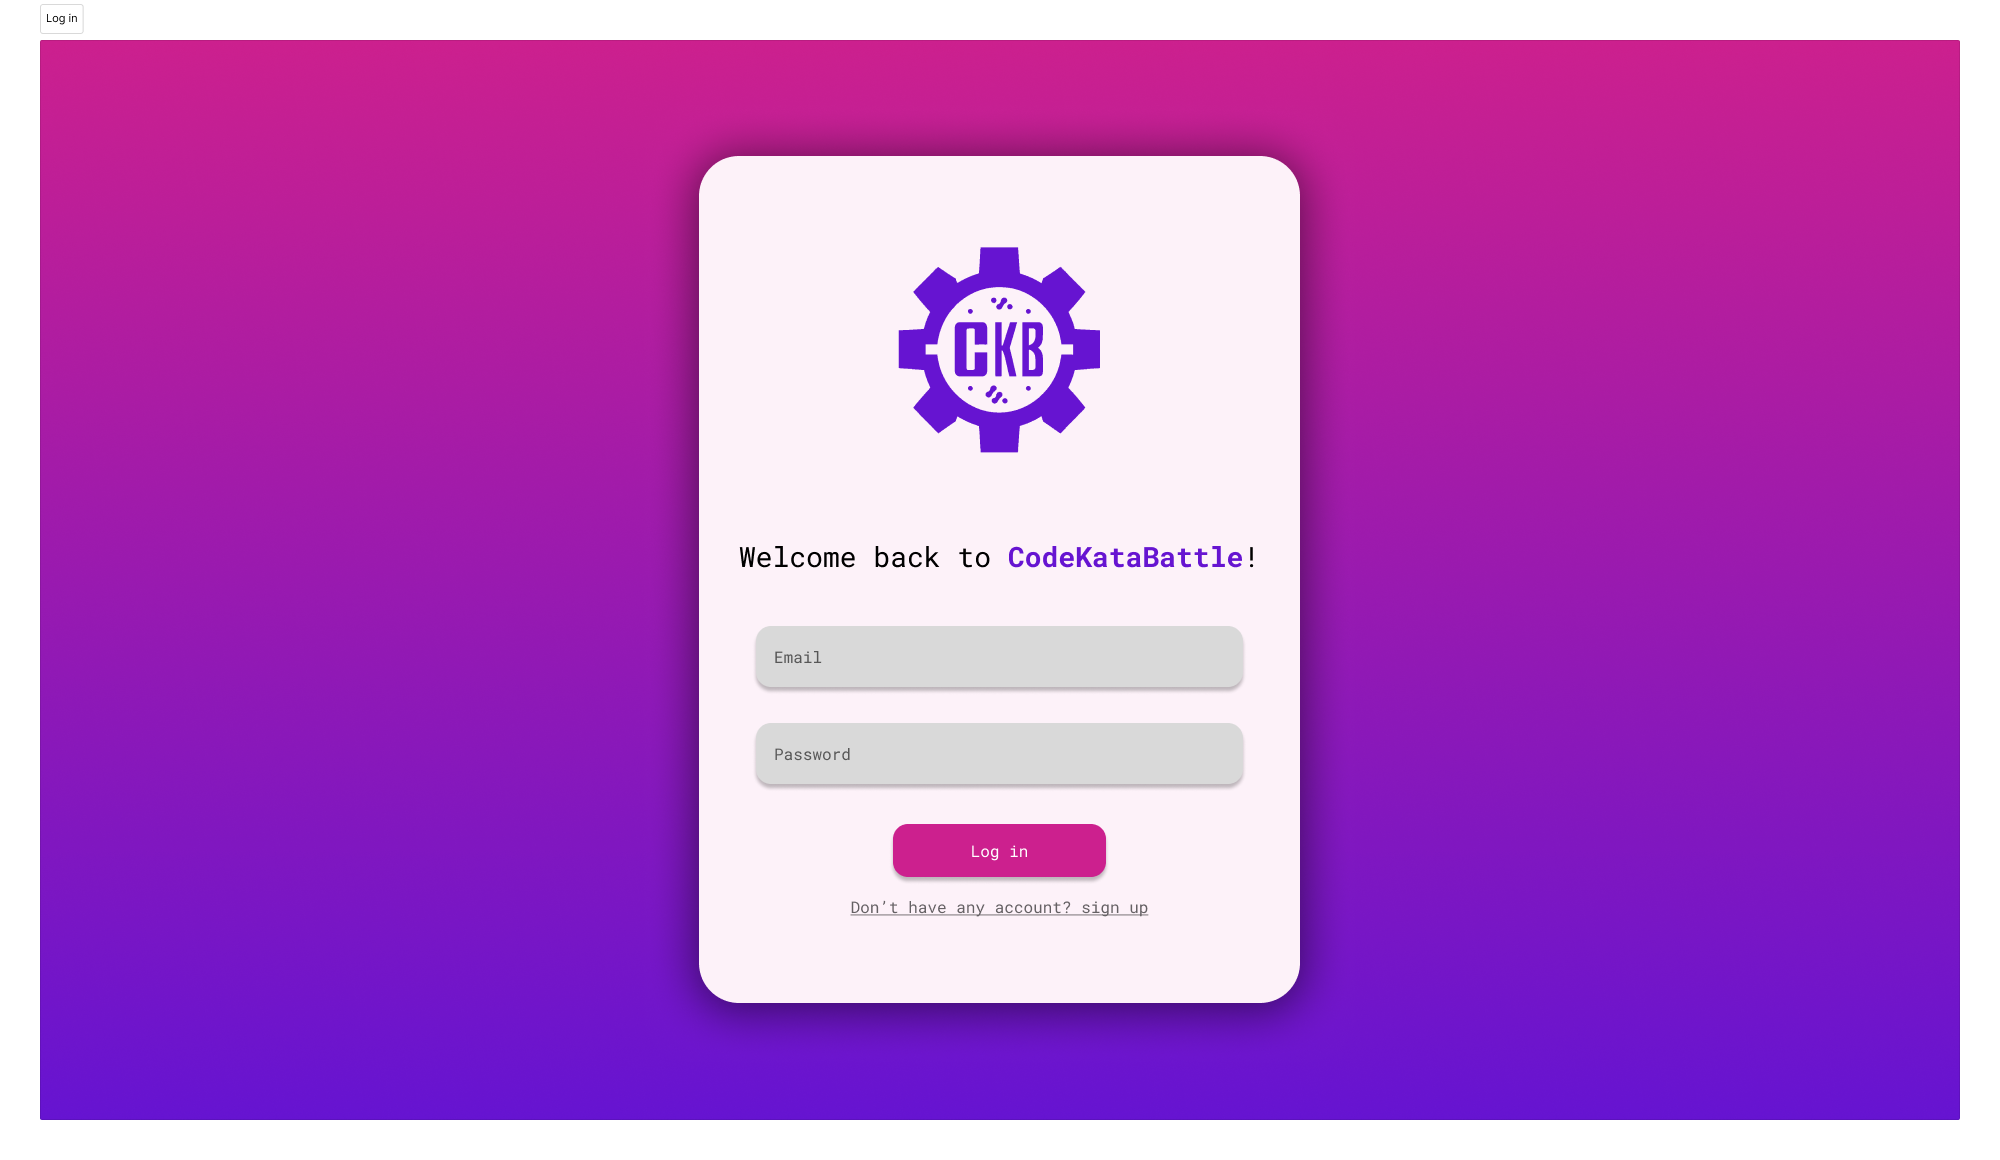
\includegraphics[width=1\textwidth]{images/user_interfaces/log_in.png}
    \caption{Log in page}
\end{figure}
\begin{figure}[H]
    \centering
    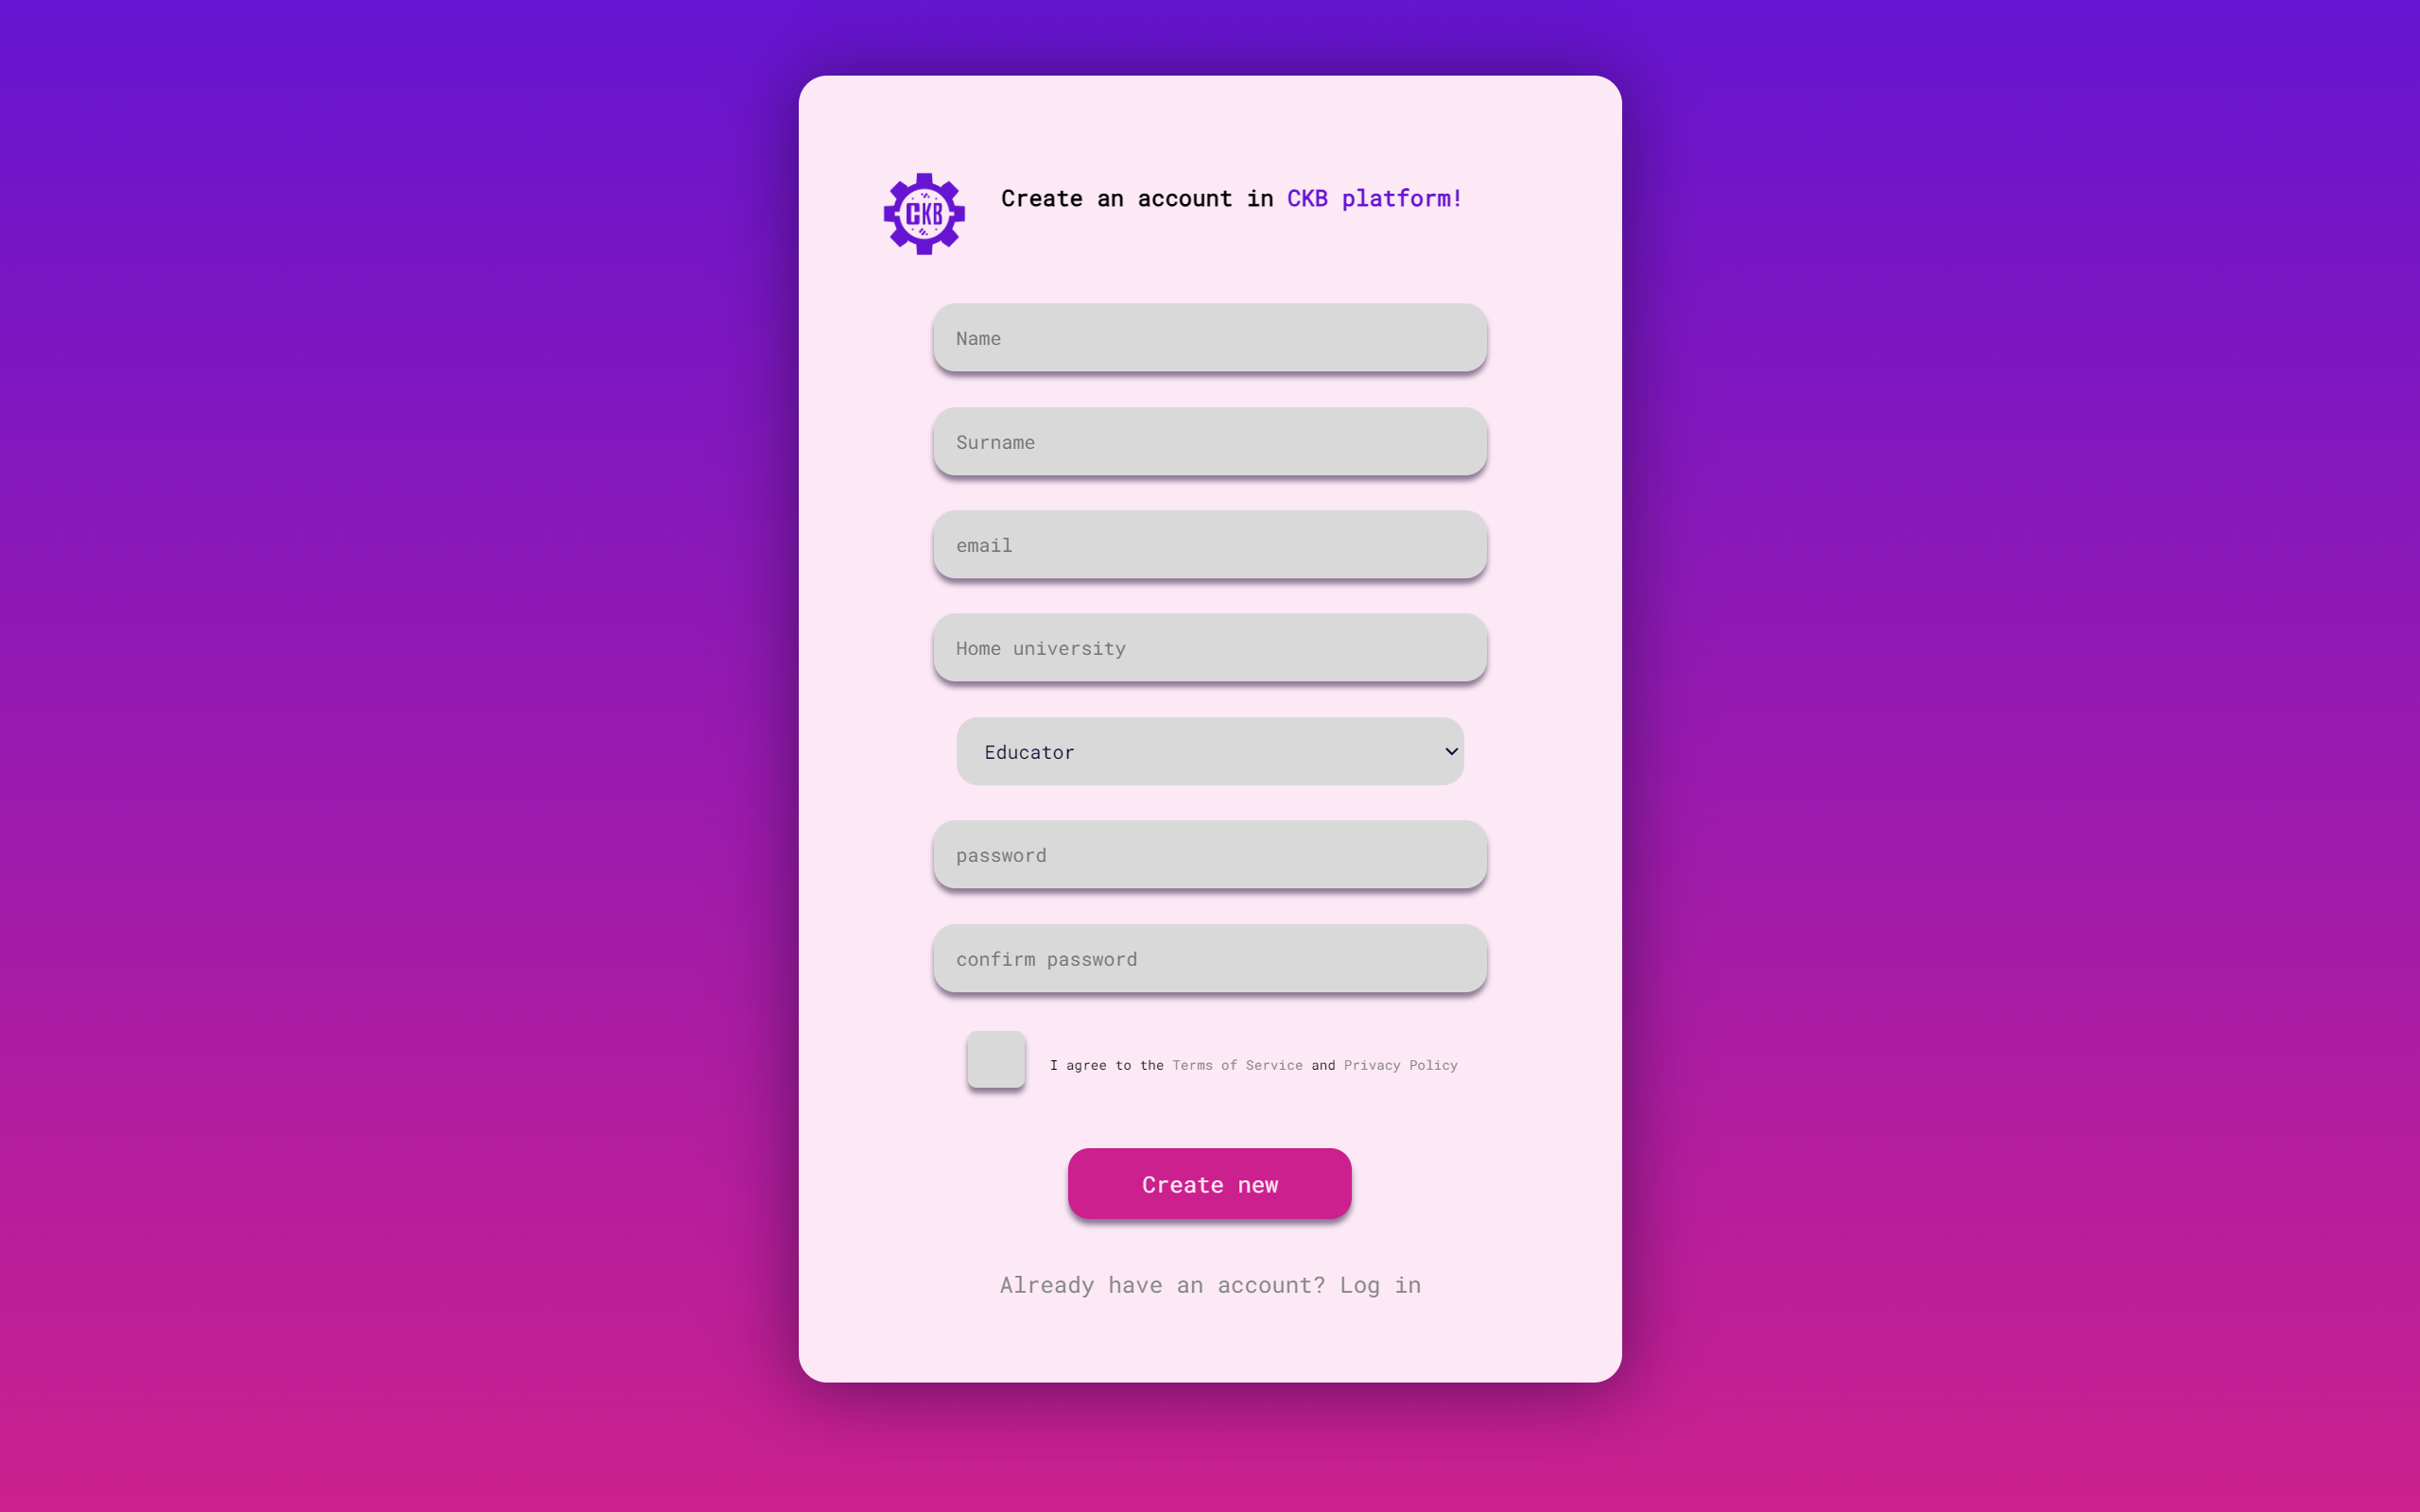
\includegraphics[width=1\textwidth]{images/user_interfaces/sign_up.png}
    \caption{Sign up page}
\end{figure}
\begin{figure}[H]
    \centering
    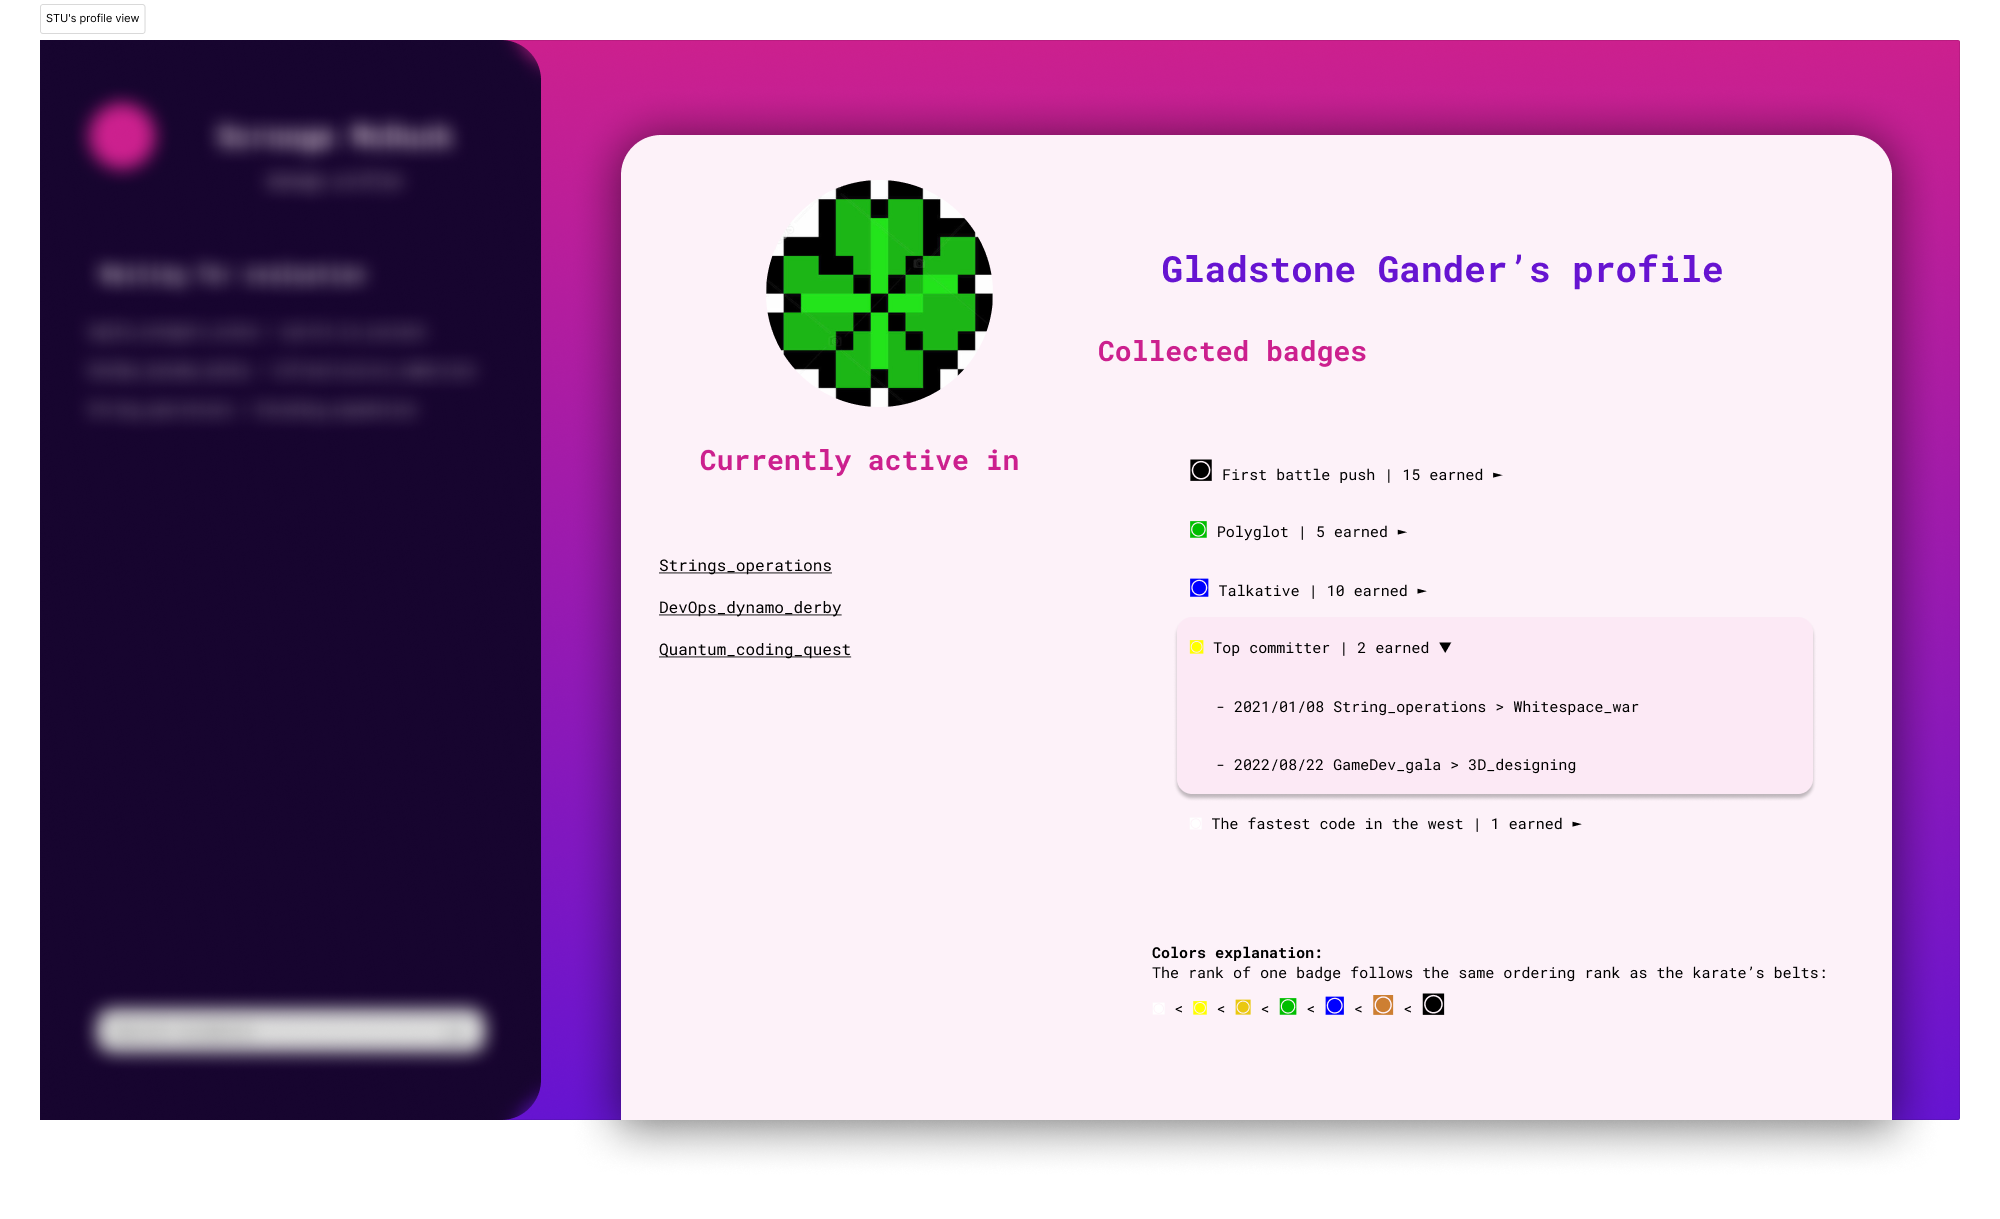
\includegraphics[width=1\textwidth]{images/user_interfaces/profile.png}
    \caption{Page that shows badges acquired by a STU}
\end{figure}

\subsubsection*{EDU's views}
\begin{figure}[H]
    \centering
    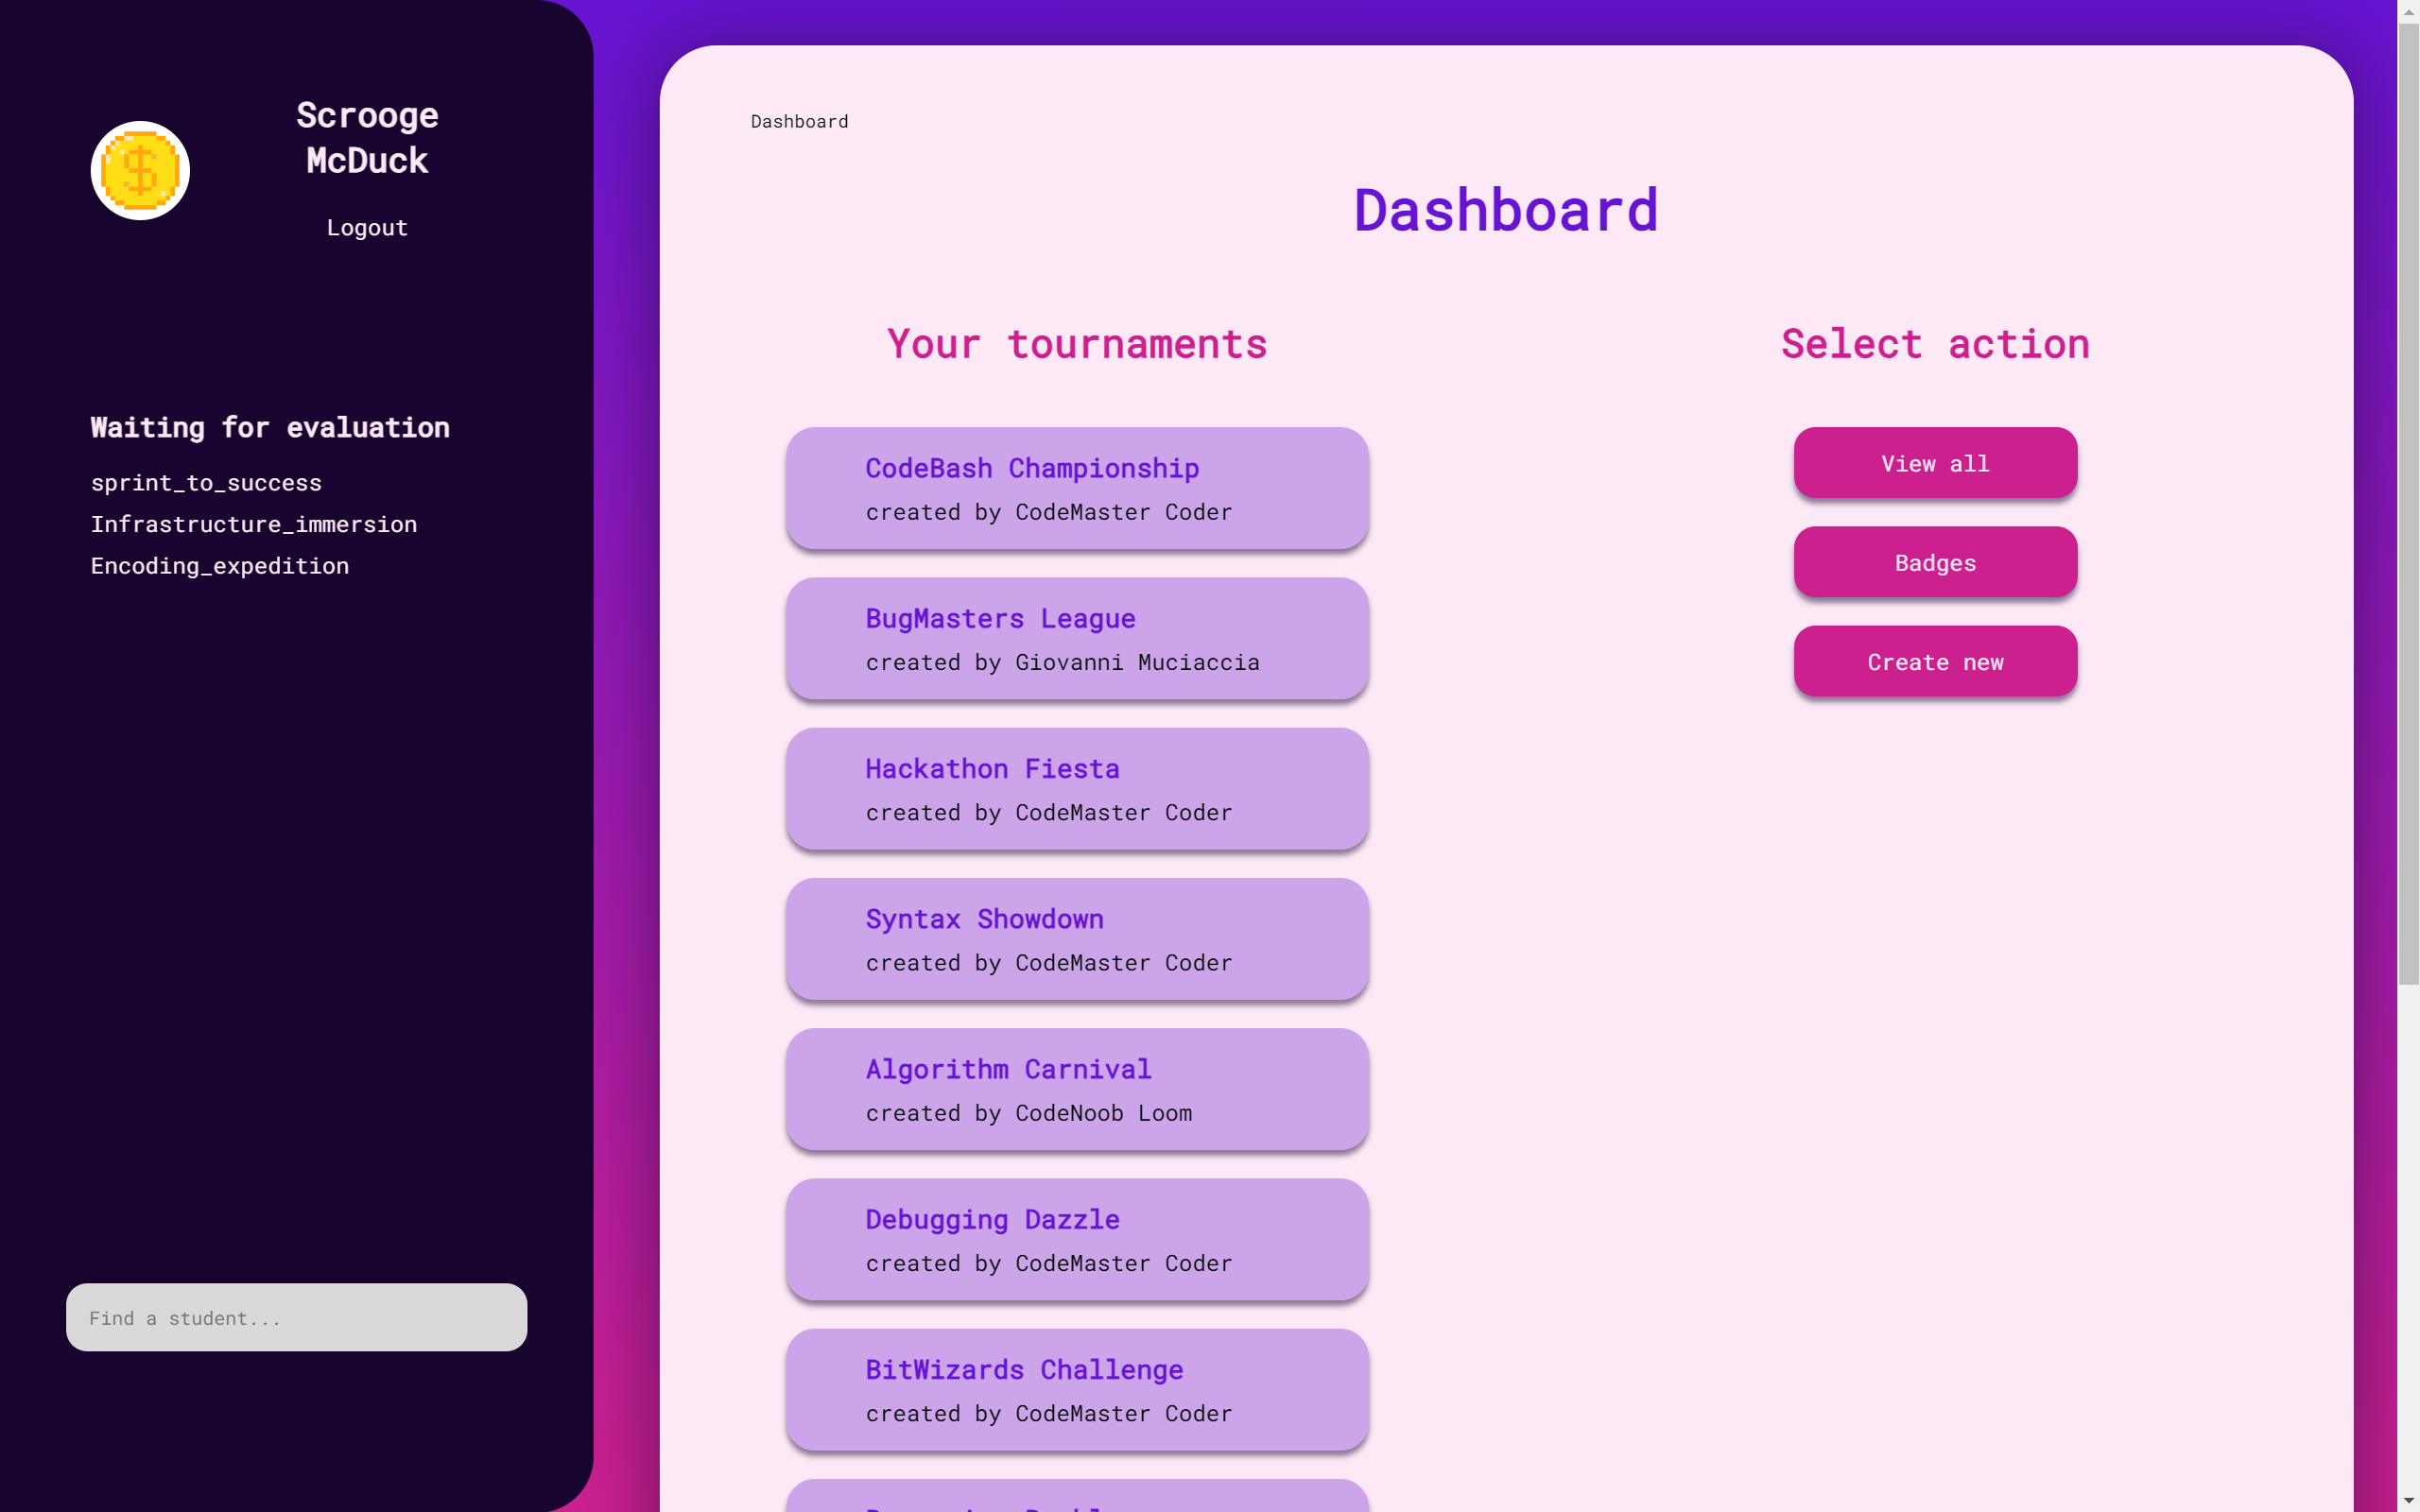
\includegraphics[width=1\textwidth]{images/user_interfaces/educator_dashboard.png}
    \caption{Dashboard}
\end{figure}
\begin{figure}[H]
    \centering
    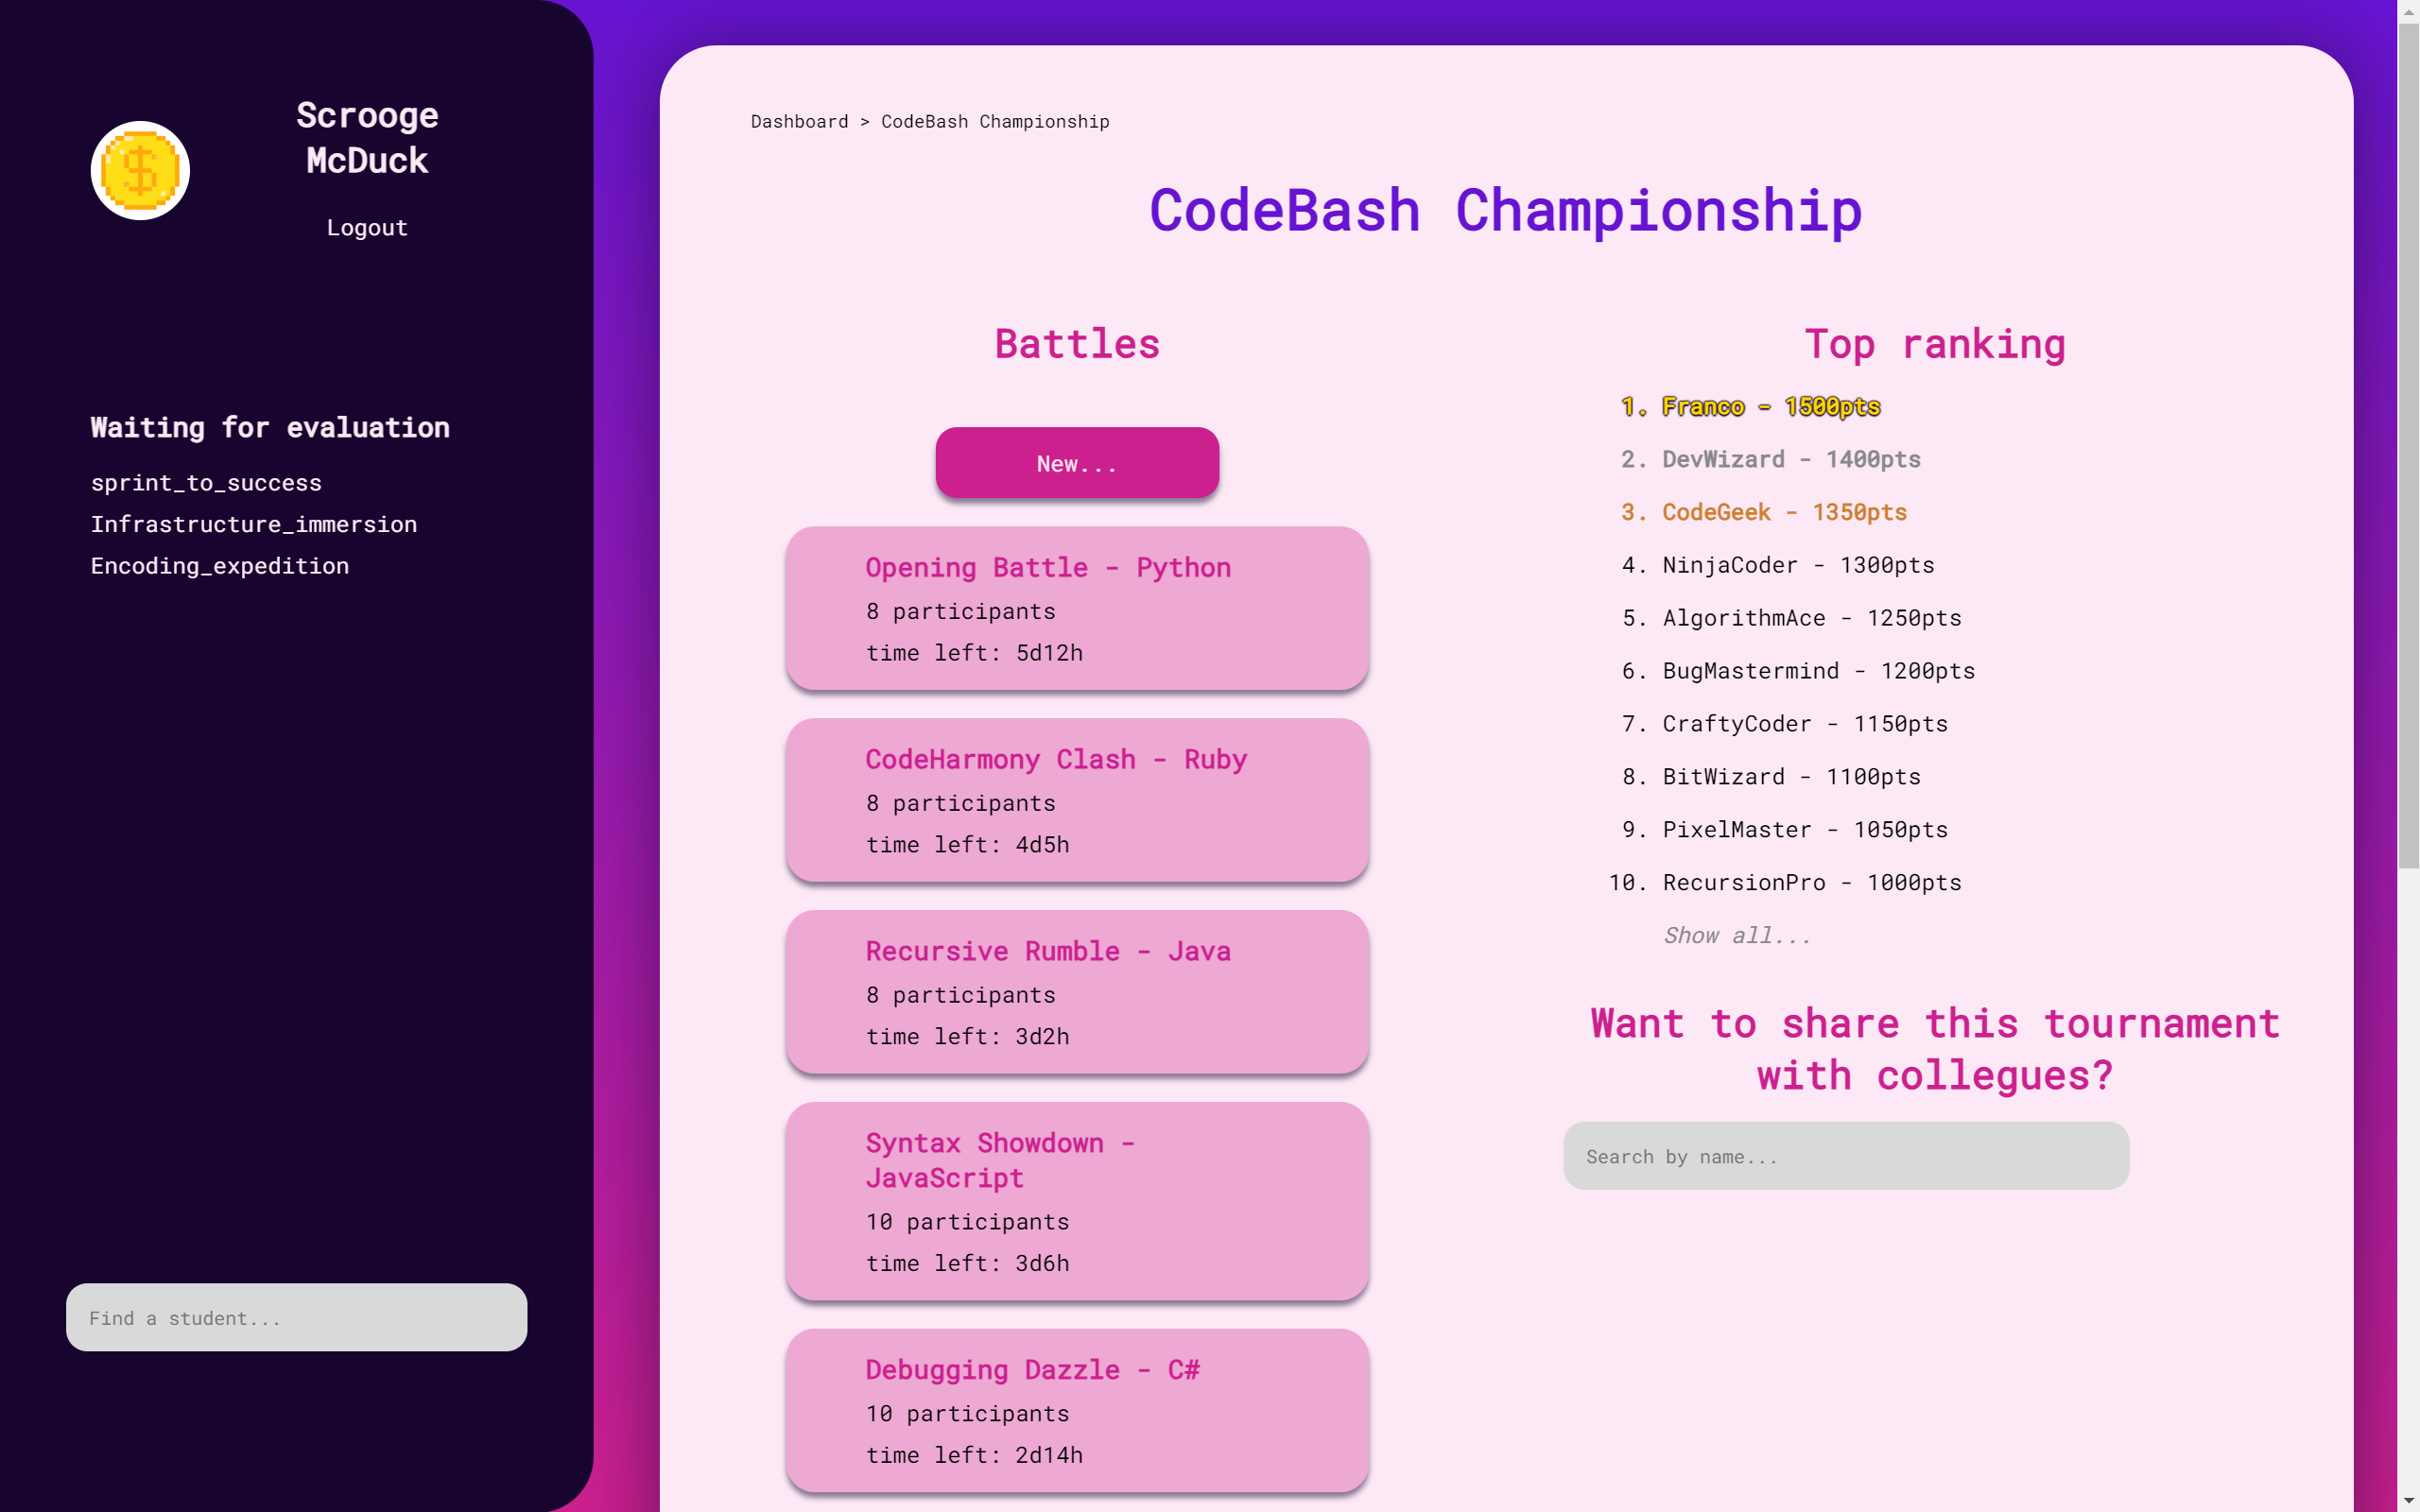
\includegraphics[width=1\textwidth]{images/user_interfaces/educator_tournament_view.png}
    \caption{View of a tournament}
\end{figure}
\begin{figure}[H]
    \centering
    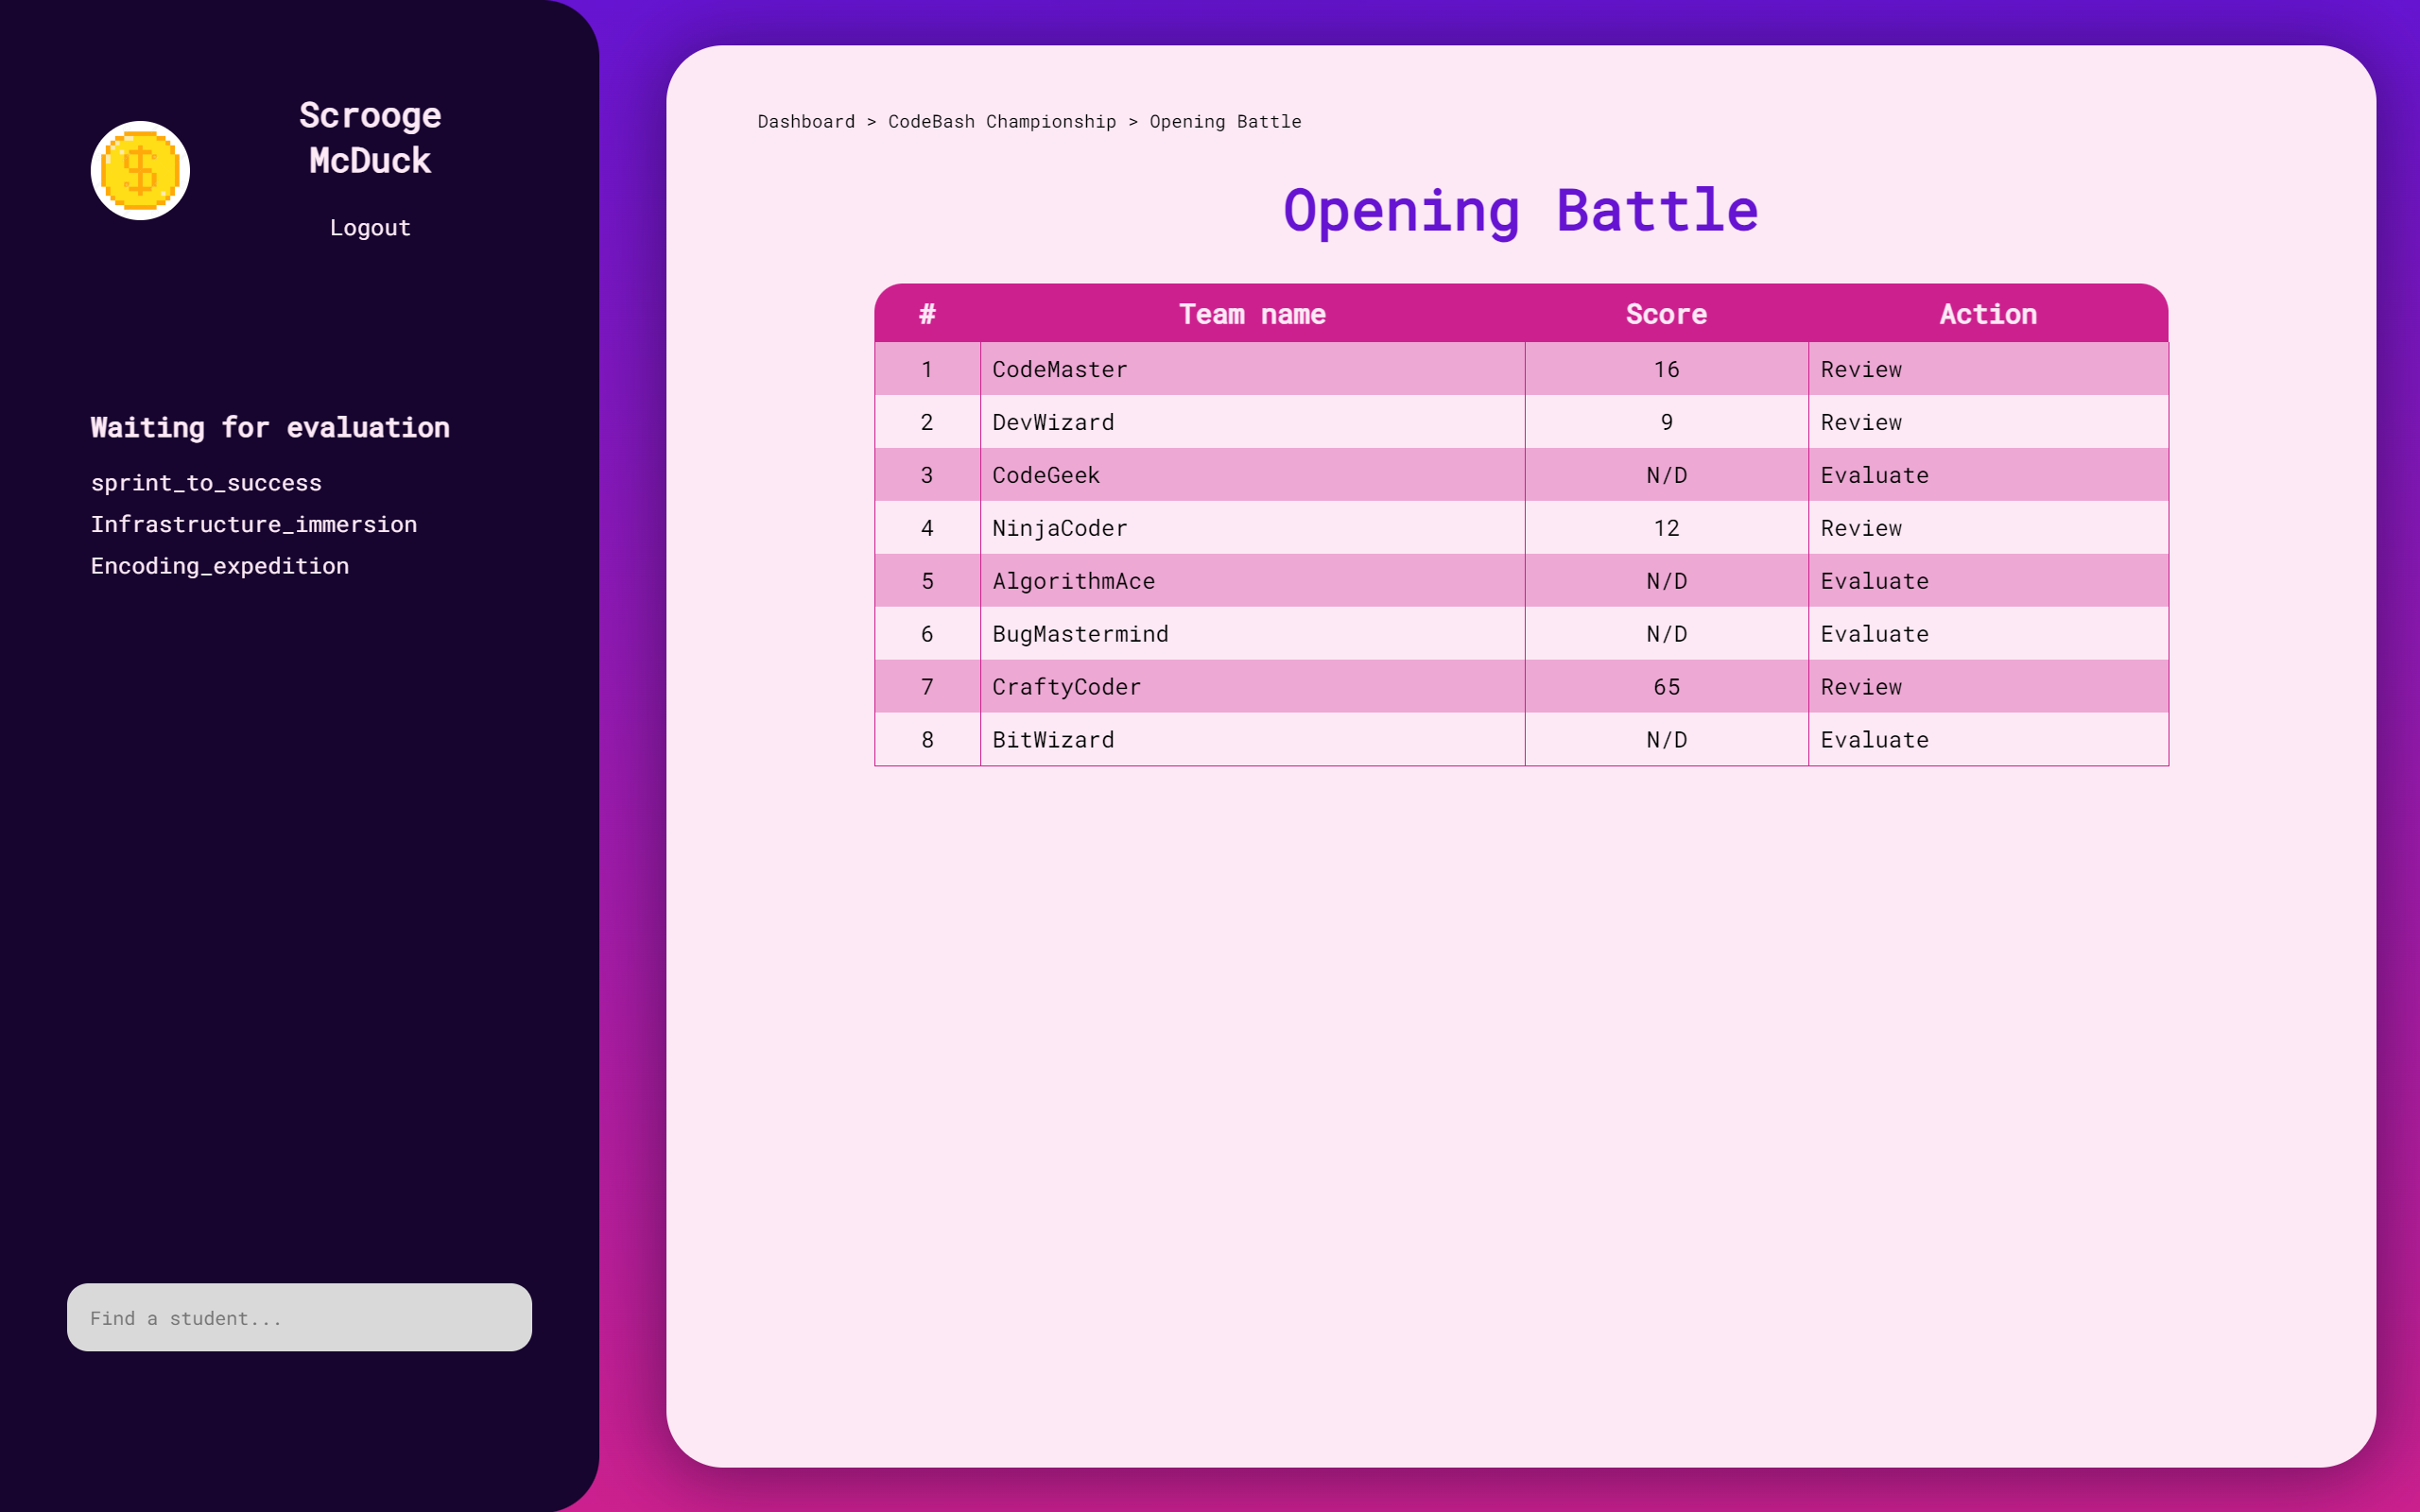
\includegraphics[width=1\textwidth]{images/user_interfaces/manual_evaluation.png}
    \caption{Manual evaluation page}
\end{figure}
\begin{figure}[H]
    \centering
    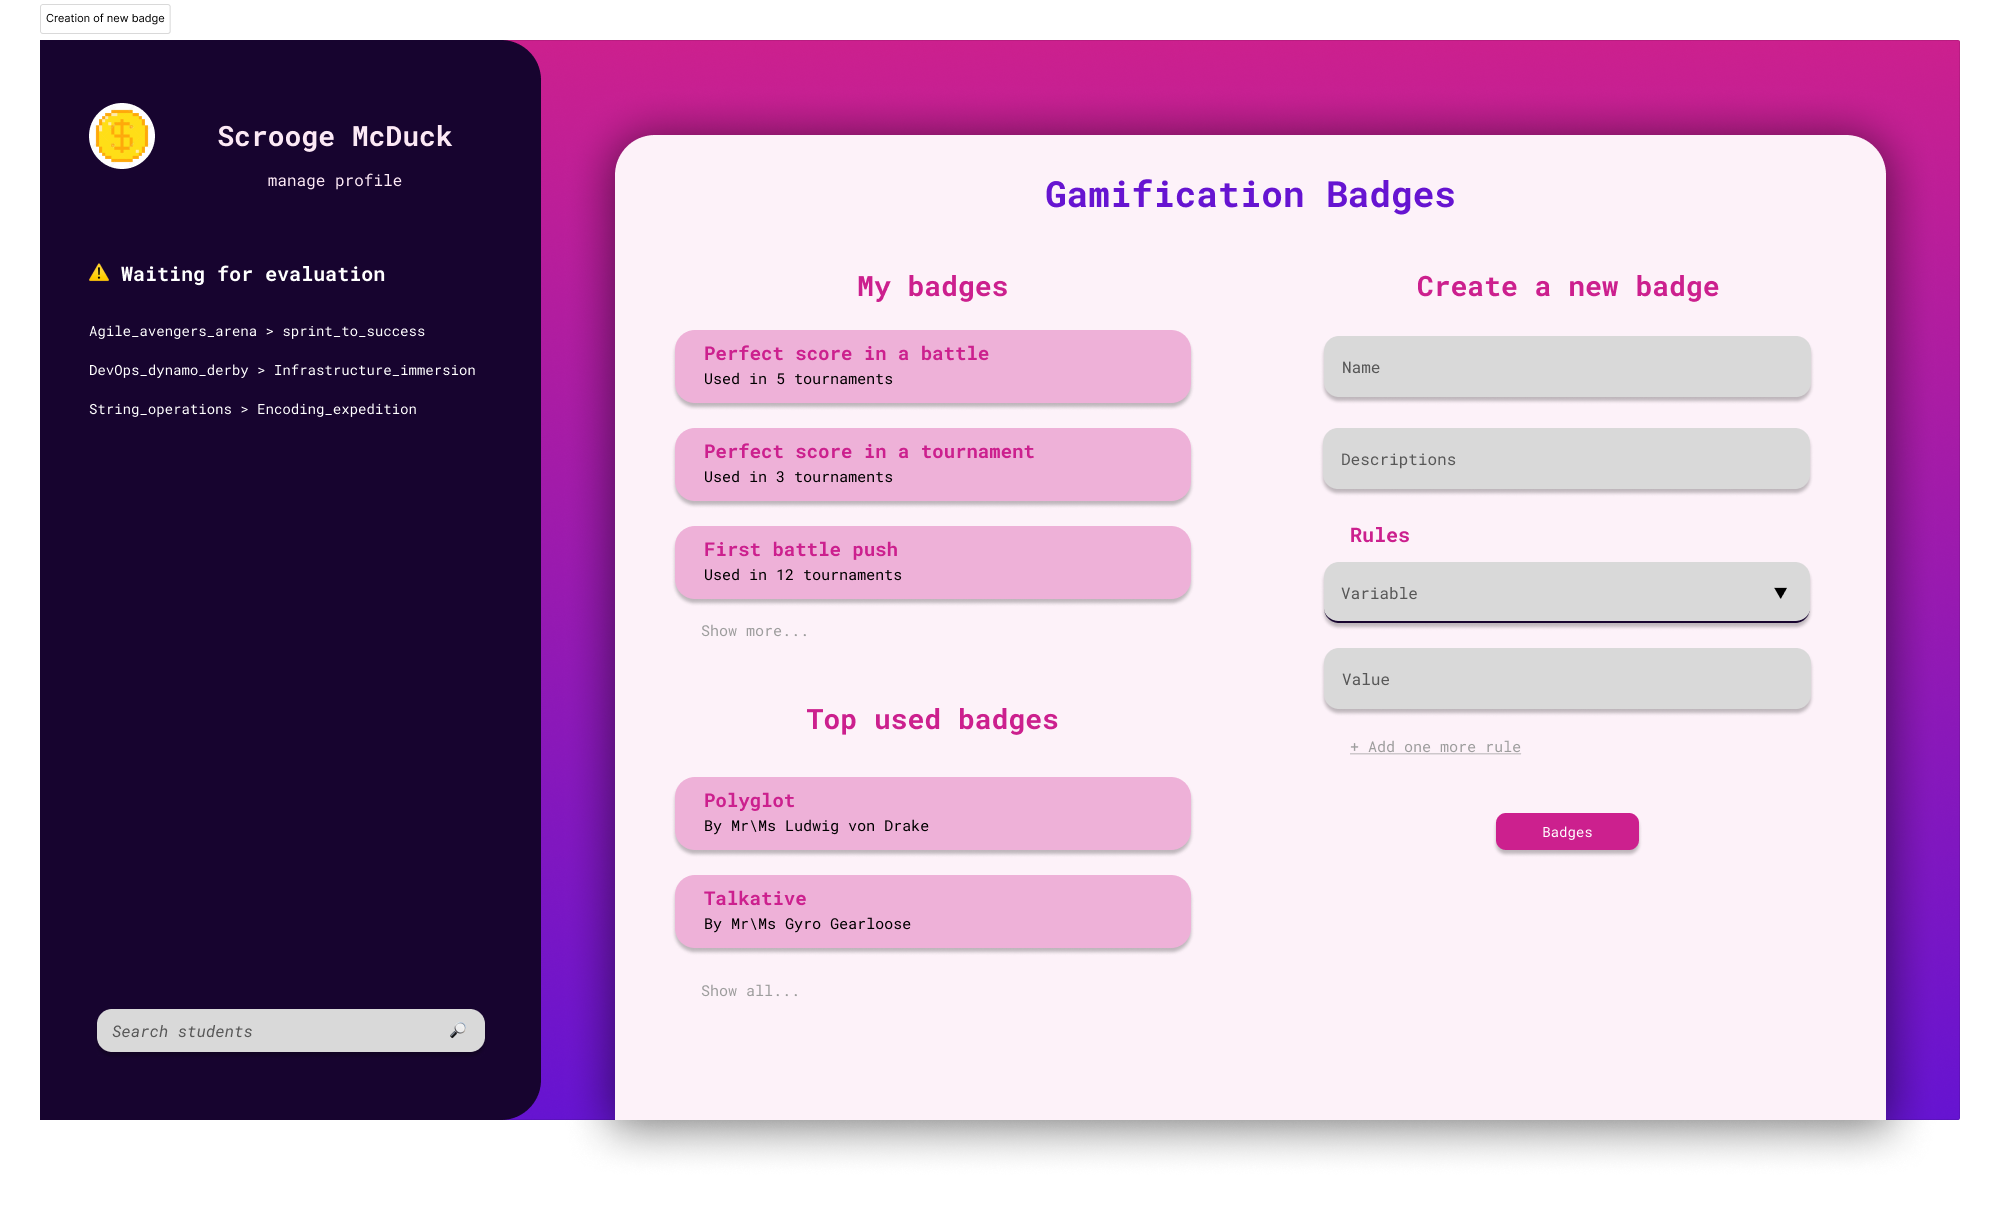
\includegraphics[width=1\textwidth]{images/user_interfaces/new_badge.png}
    \caption{Page to create a new badge}
\end{figure}

\subsubsection*{STU's views}
\begin{figure}[H]
    \centering
    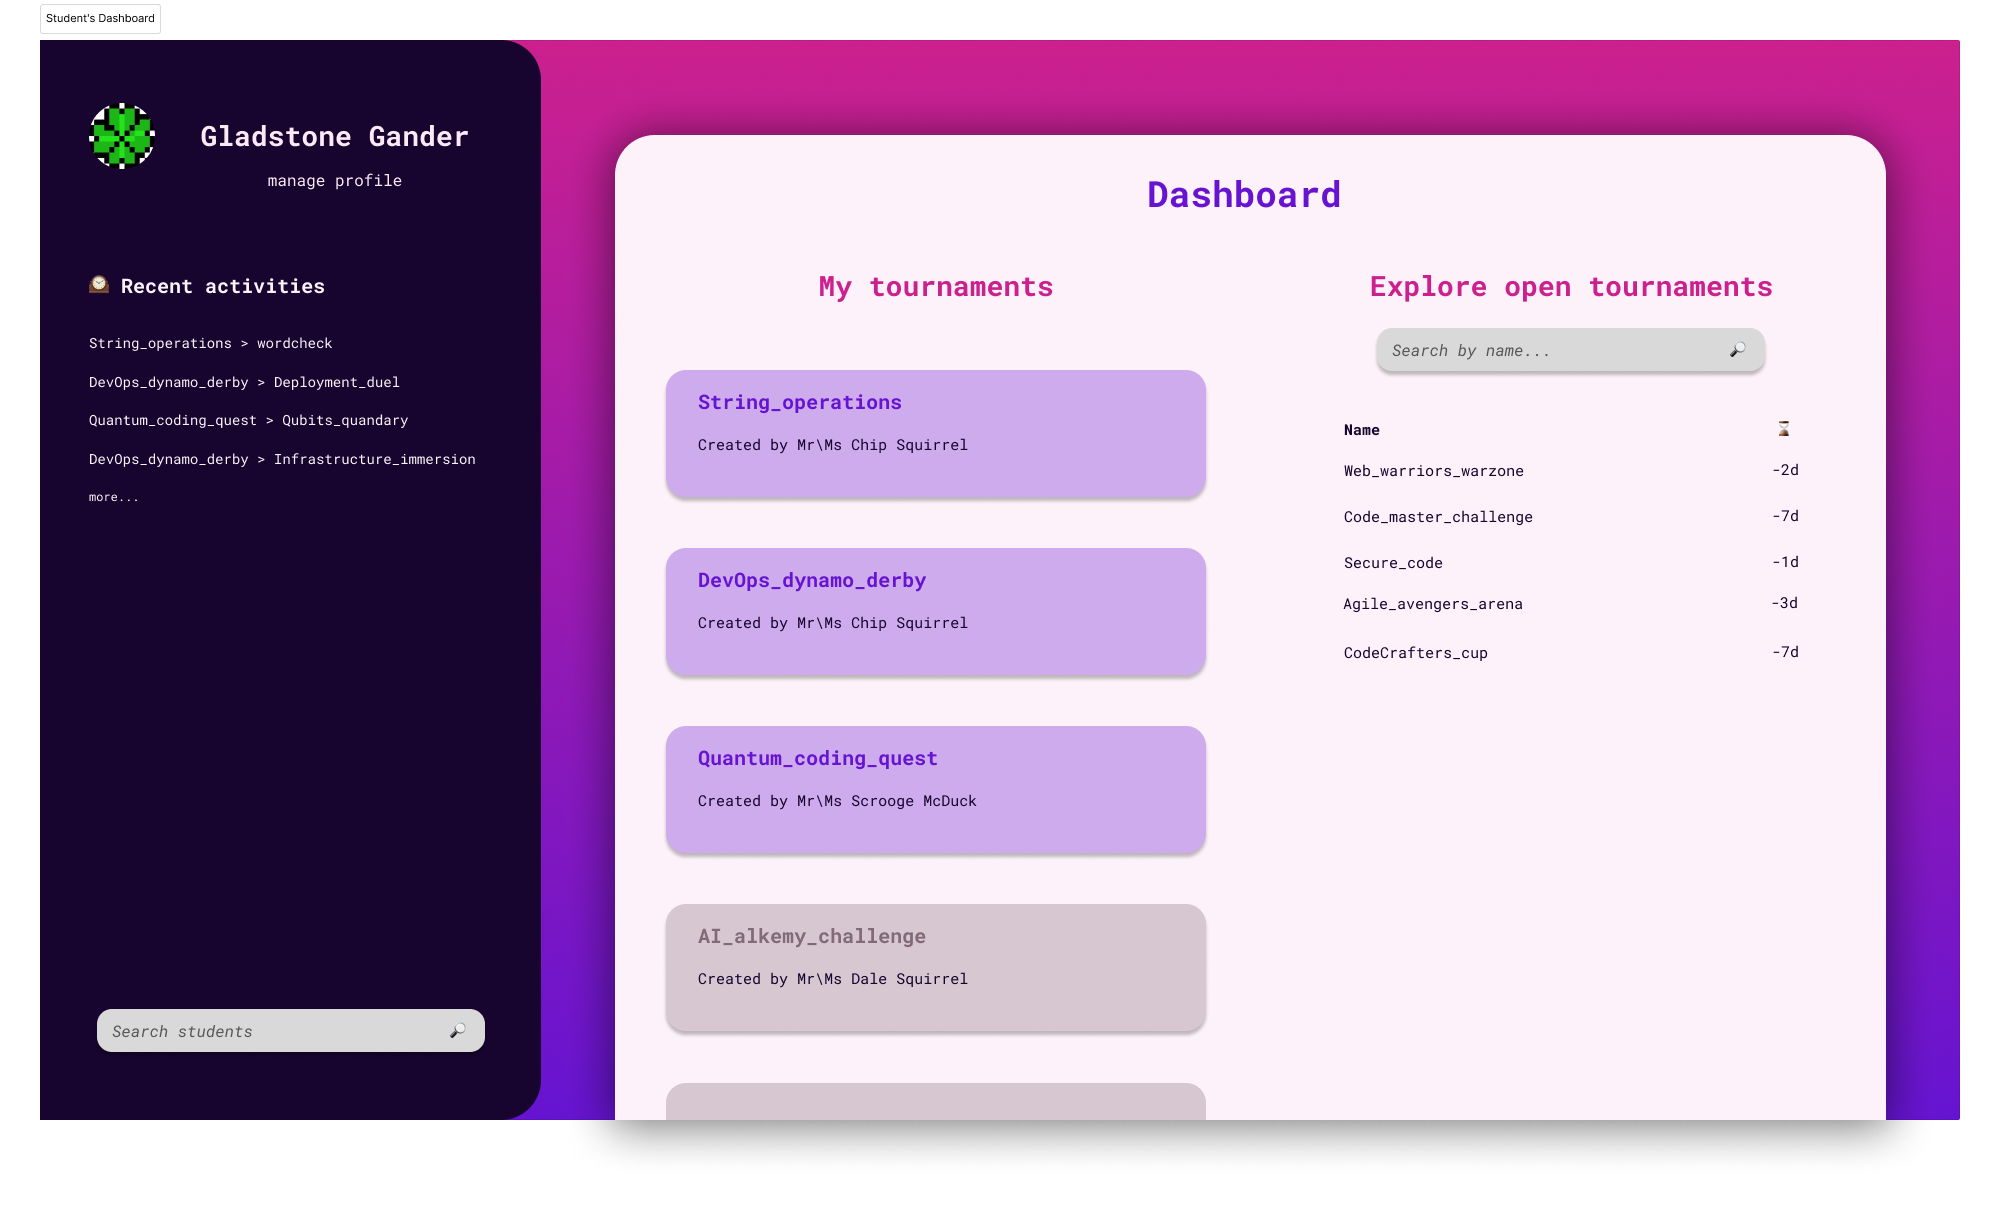
\includegraphics[width=1\textwidth]{images/user_interfaces/student_dashboard.png}
    \caption{Dashboard}
\end{figure}
\begin{figure}[H]
    \centering
    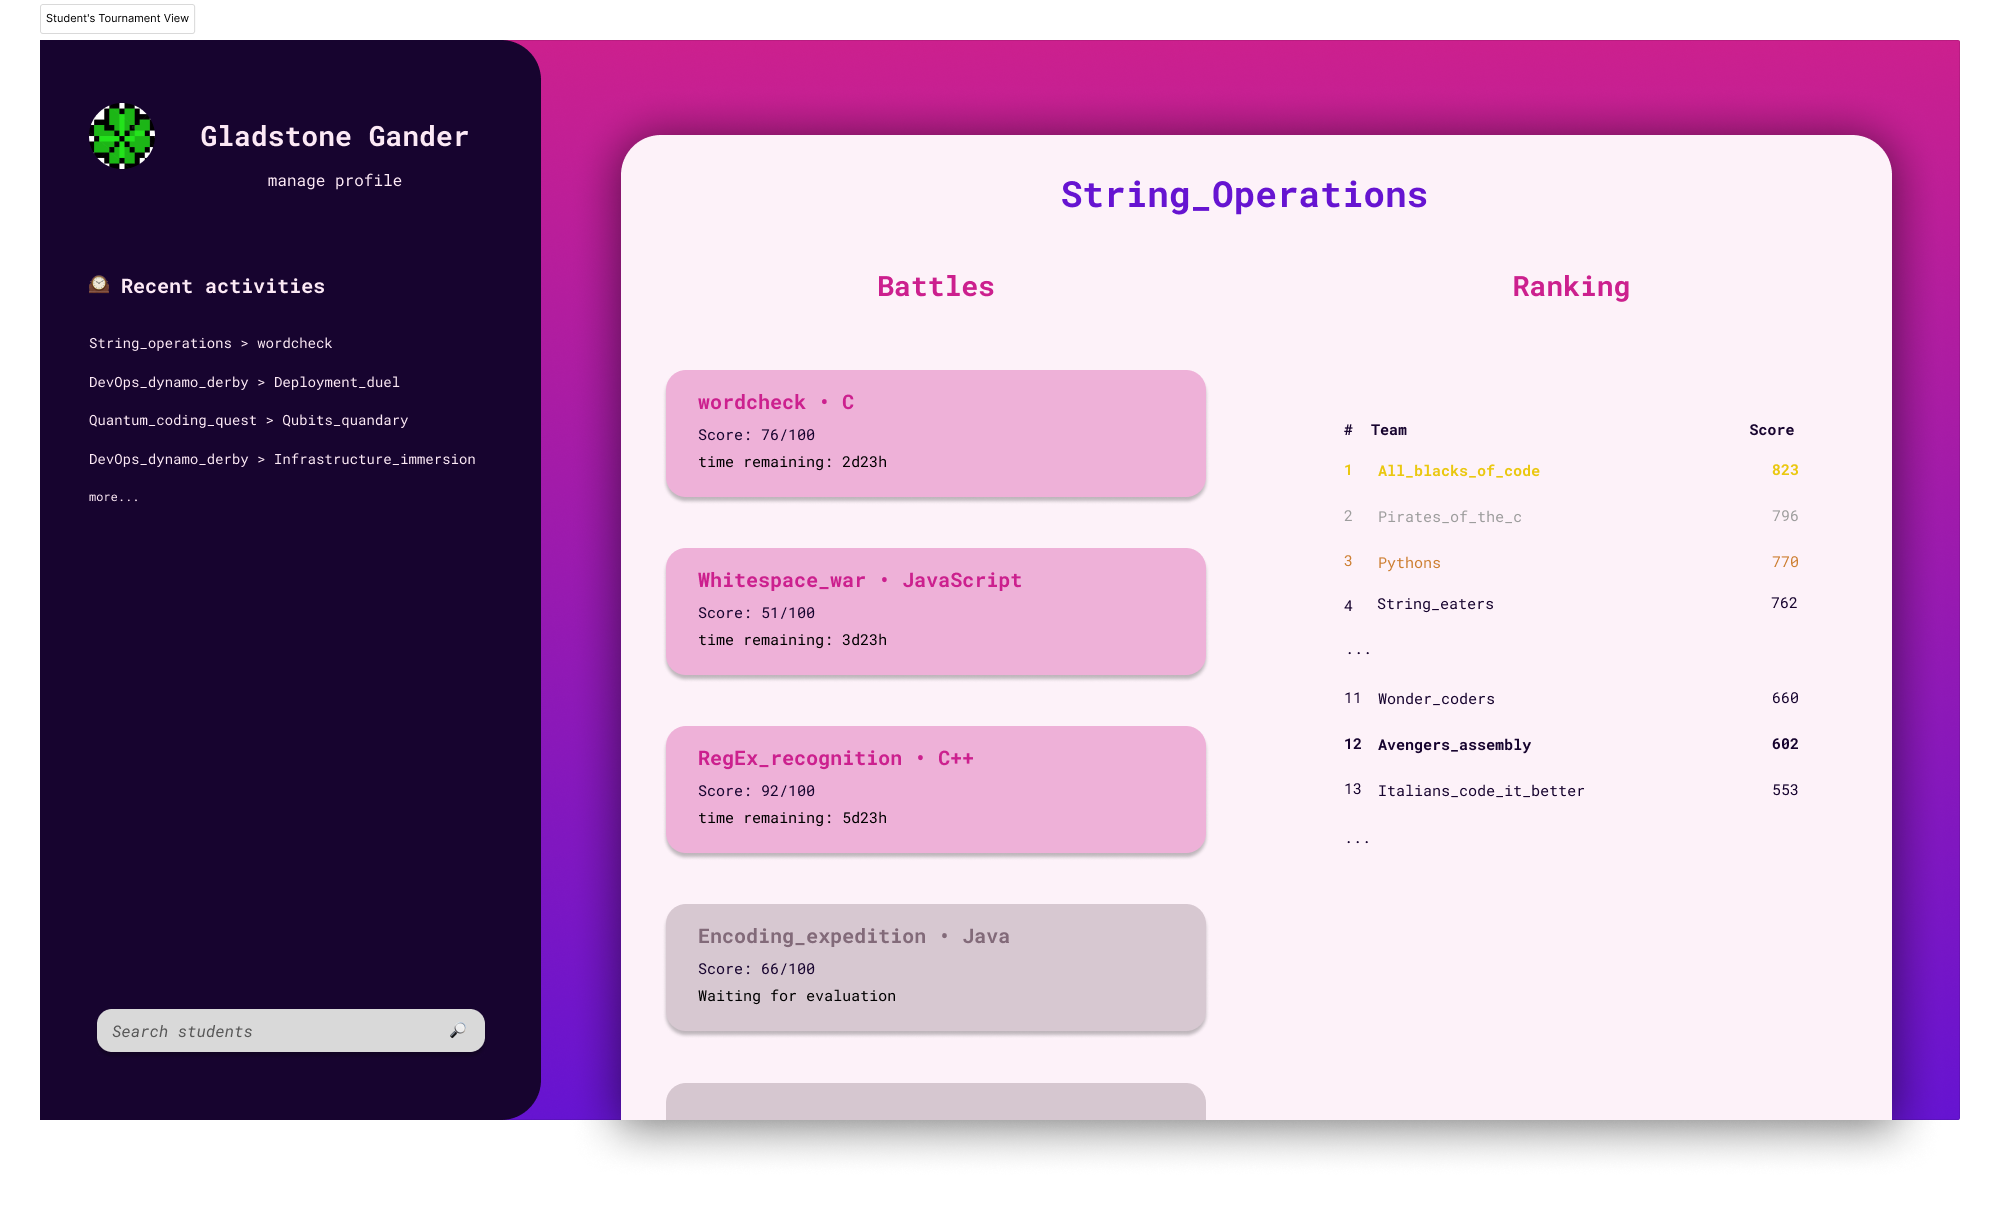
\includegraphics[width=1\textwidth]{images/user_interfaces/student_tournament_view.png}
    \caption{View of a tournament}
\end{figure}
\begin{figure}[H]
    \centering
    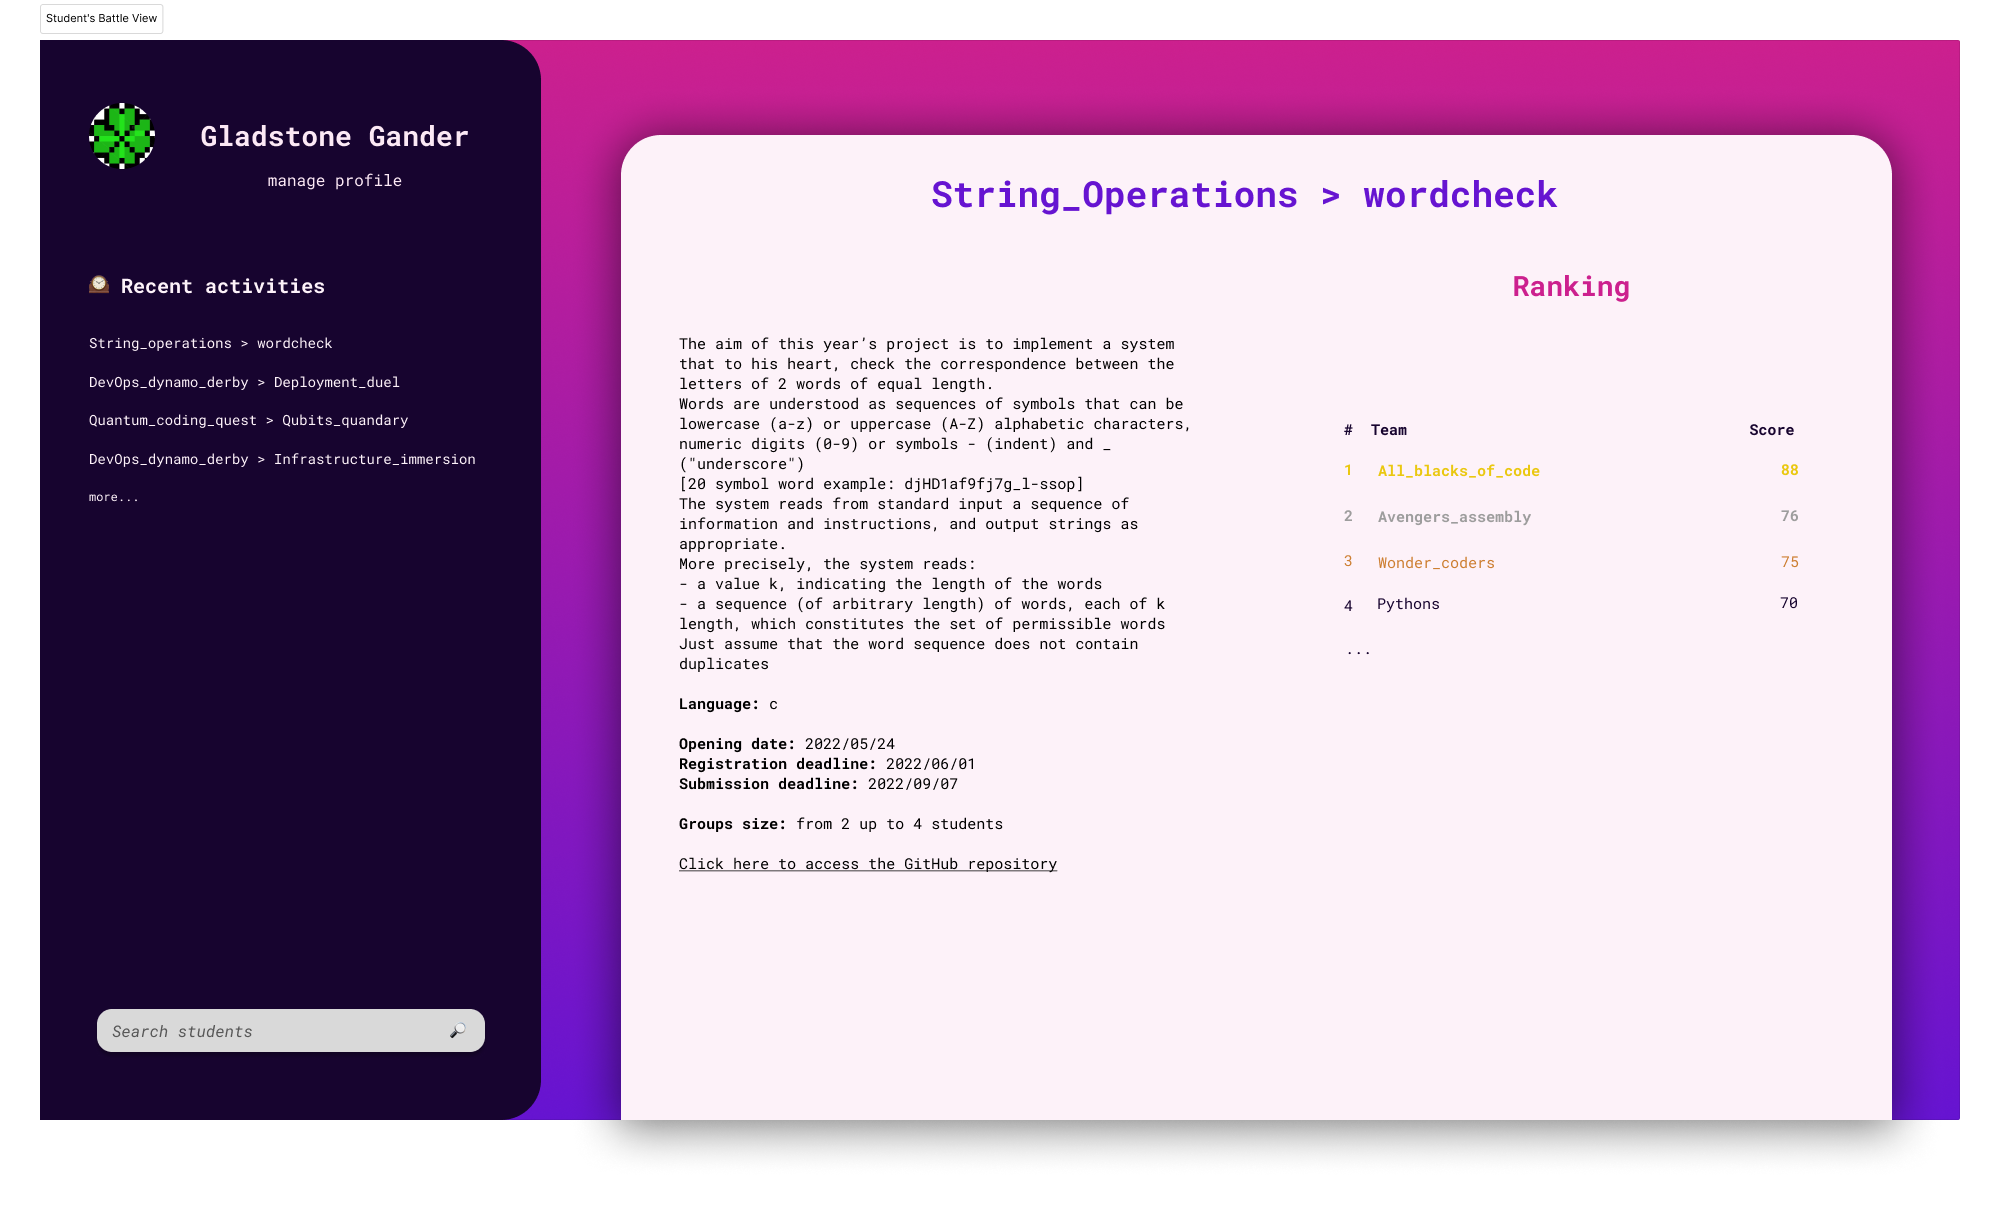
\includegraphics[width=1\textwidth]{images/user_interfaces/student_battle_view.png}
    \caption{View of a battle}
\end{figure}

\subsection{Hardware Interfaces}
To use the CKB platform, both the Educators and the Students need an electronic device connected to the Internet, like a computer, a tablet, or a smartphone.\\
As the platform's primary functionality is closely tied to coding activities, it is expected that users will predominantly employ personal computers to access an Integrated Development Environment (IDE).
Consequently, the platform's interfaces have been optimized for use on computer screens.

\subsection{Software Interfaces}
Since the platform is web-based, it is compatible with all the major operating systems, as long as they have a modern browser installed.

\subsection{Communication Interfaces}
The system requires a stable internet connection to work properly.
The backend of the system will expose a unified RESTful API to communicate with all clients.\\
Furthermore, the system relies on various external interfaces accessible via uniform web API.
These services are:
\begin{itemize}
    \item \textbf{GitHub API:} to create and manage repositories and to retrieve students' code.
    \item \textbf{Mail API:} to send emails to the users to notify them about events.
\end{itemize}

\section{Functional Requirements}
To work properly, the software must fulfill the following functional requirements, which are written in hierarchical order, starting from those about EDUs and then STUs.

\subsection{Use cases Diagrams}
\begin{figure}[H]
    \centering
    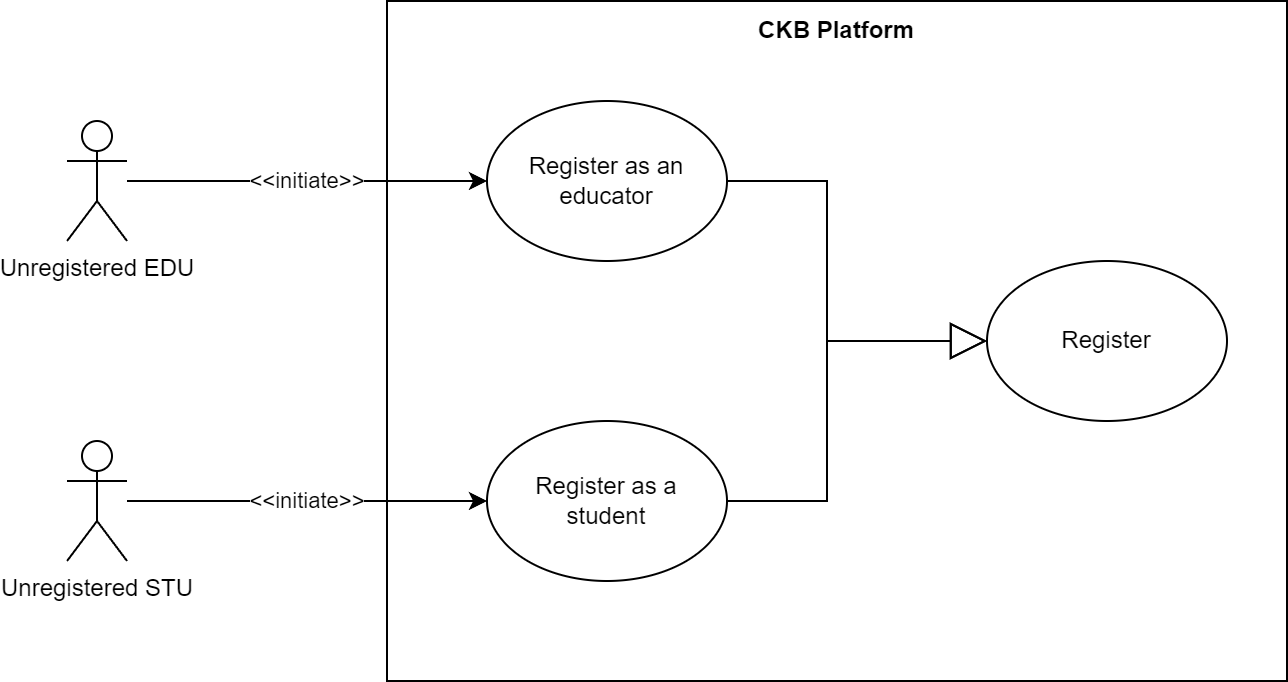
\includegraphics[width=0.8\textwidth]{images/sequence_diagrams/use_case_diagrams_registration.png}
    \caption{Registration Use Case Diagram}
\end{figure}

\begin{figure}[H]
    \centering
    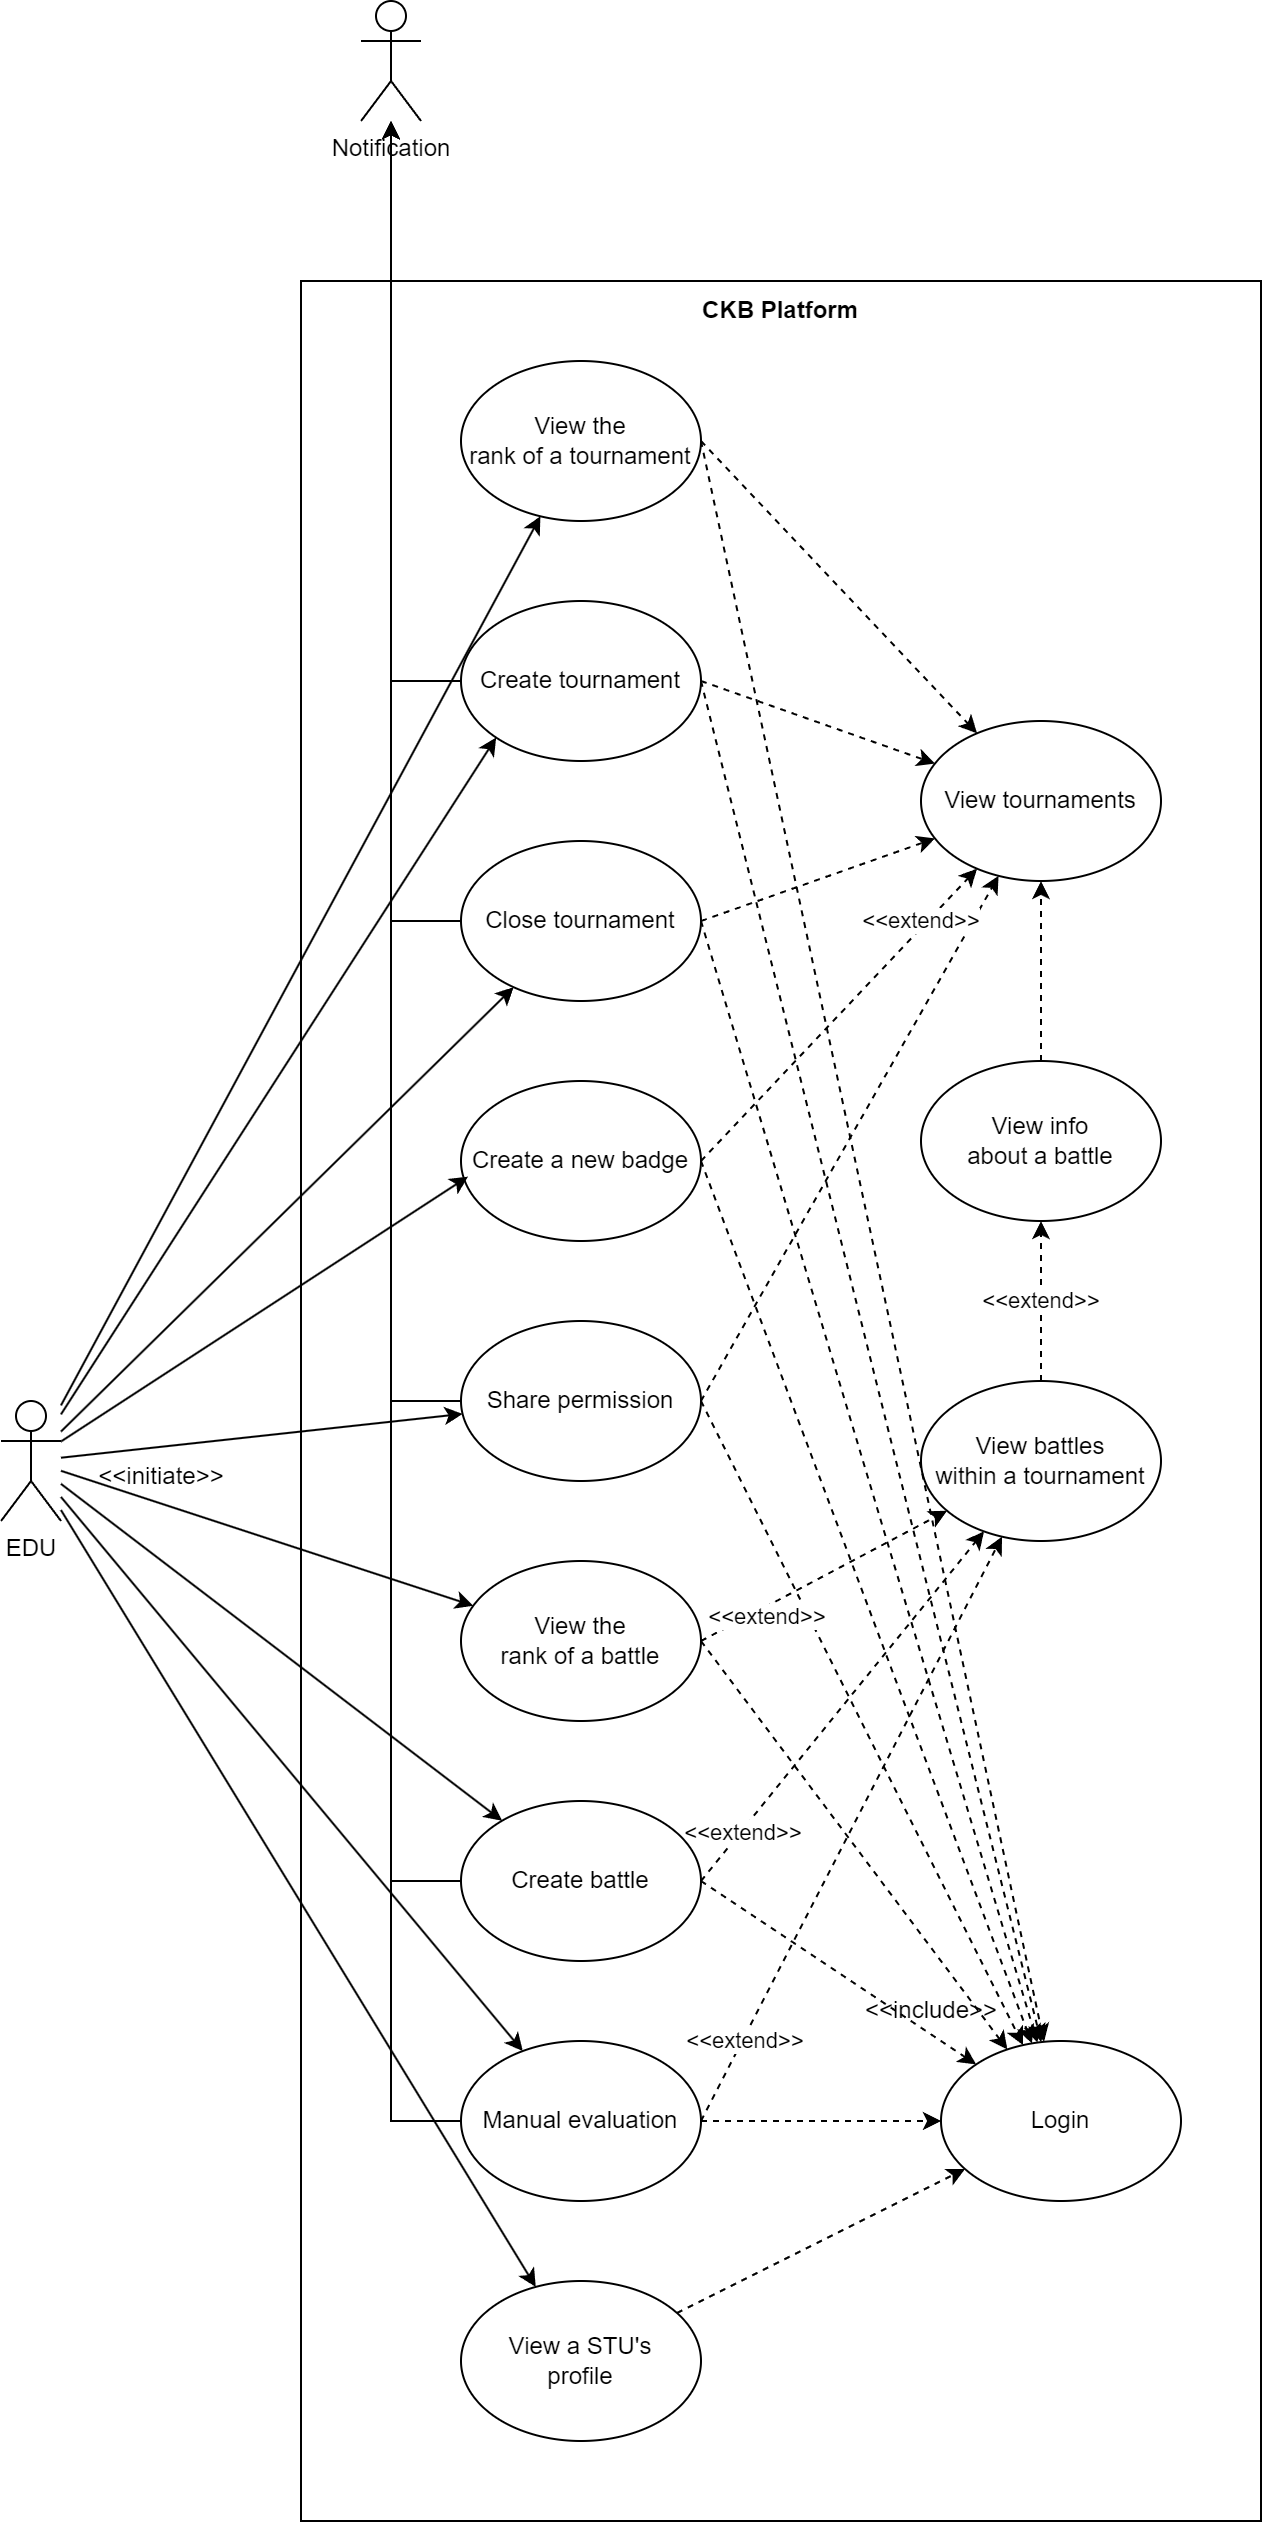
\includegraphics[width=0.6\textwidth]{images/sequence_diagrams/use_case_diagrams_EDU.png}
    \caption{EDU Use Case Diagram}
\end{figure}

\begin{figure}[H]
    \centering
    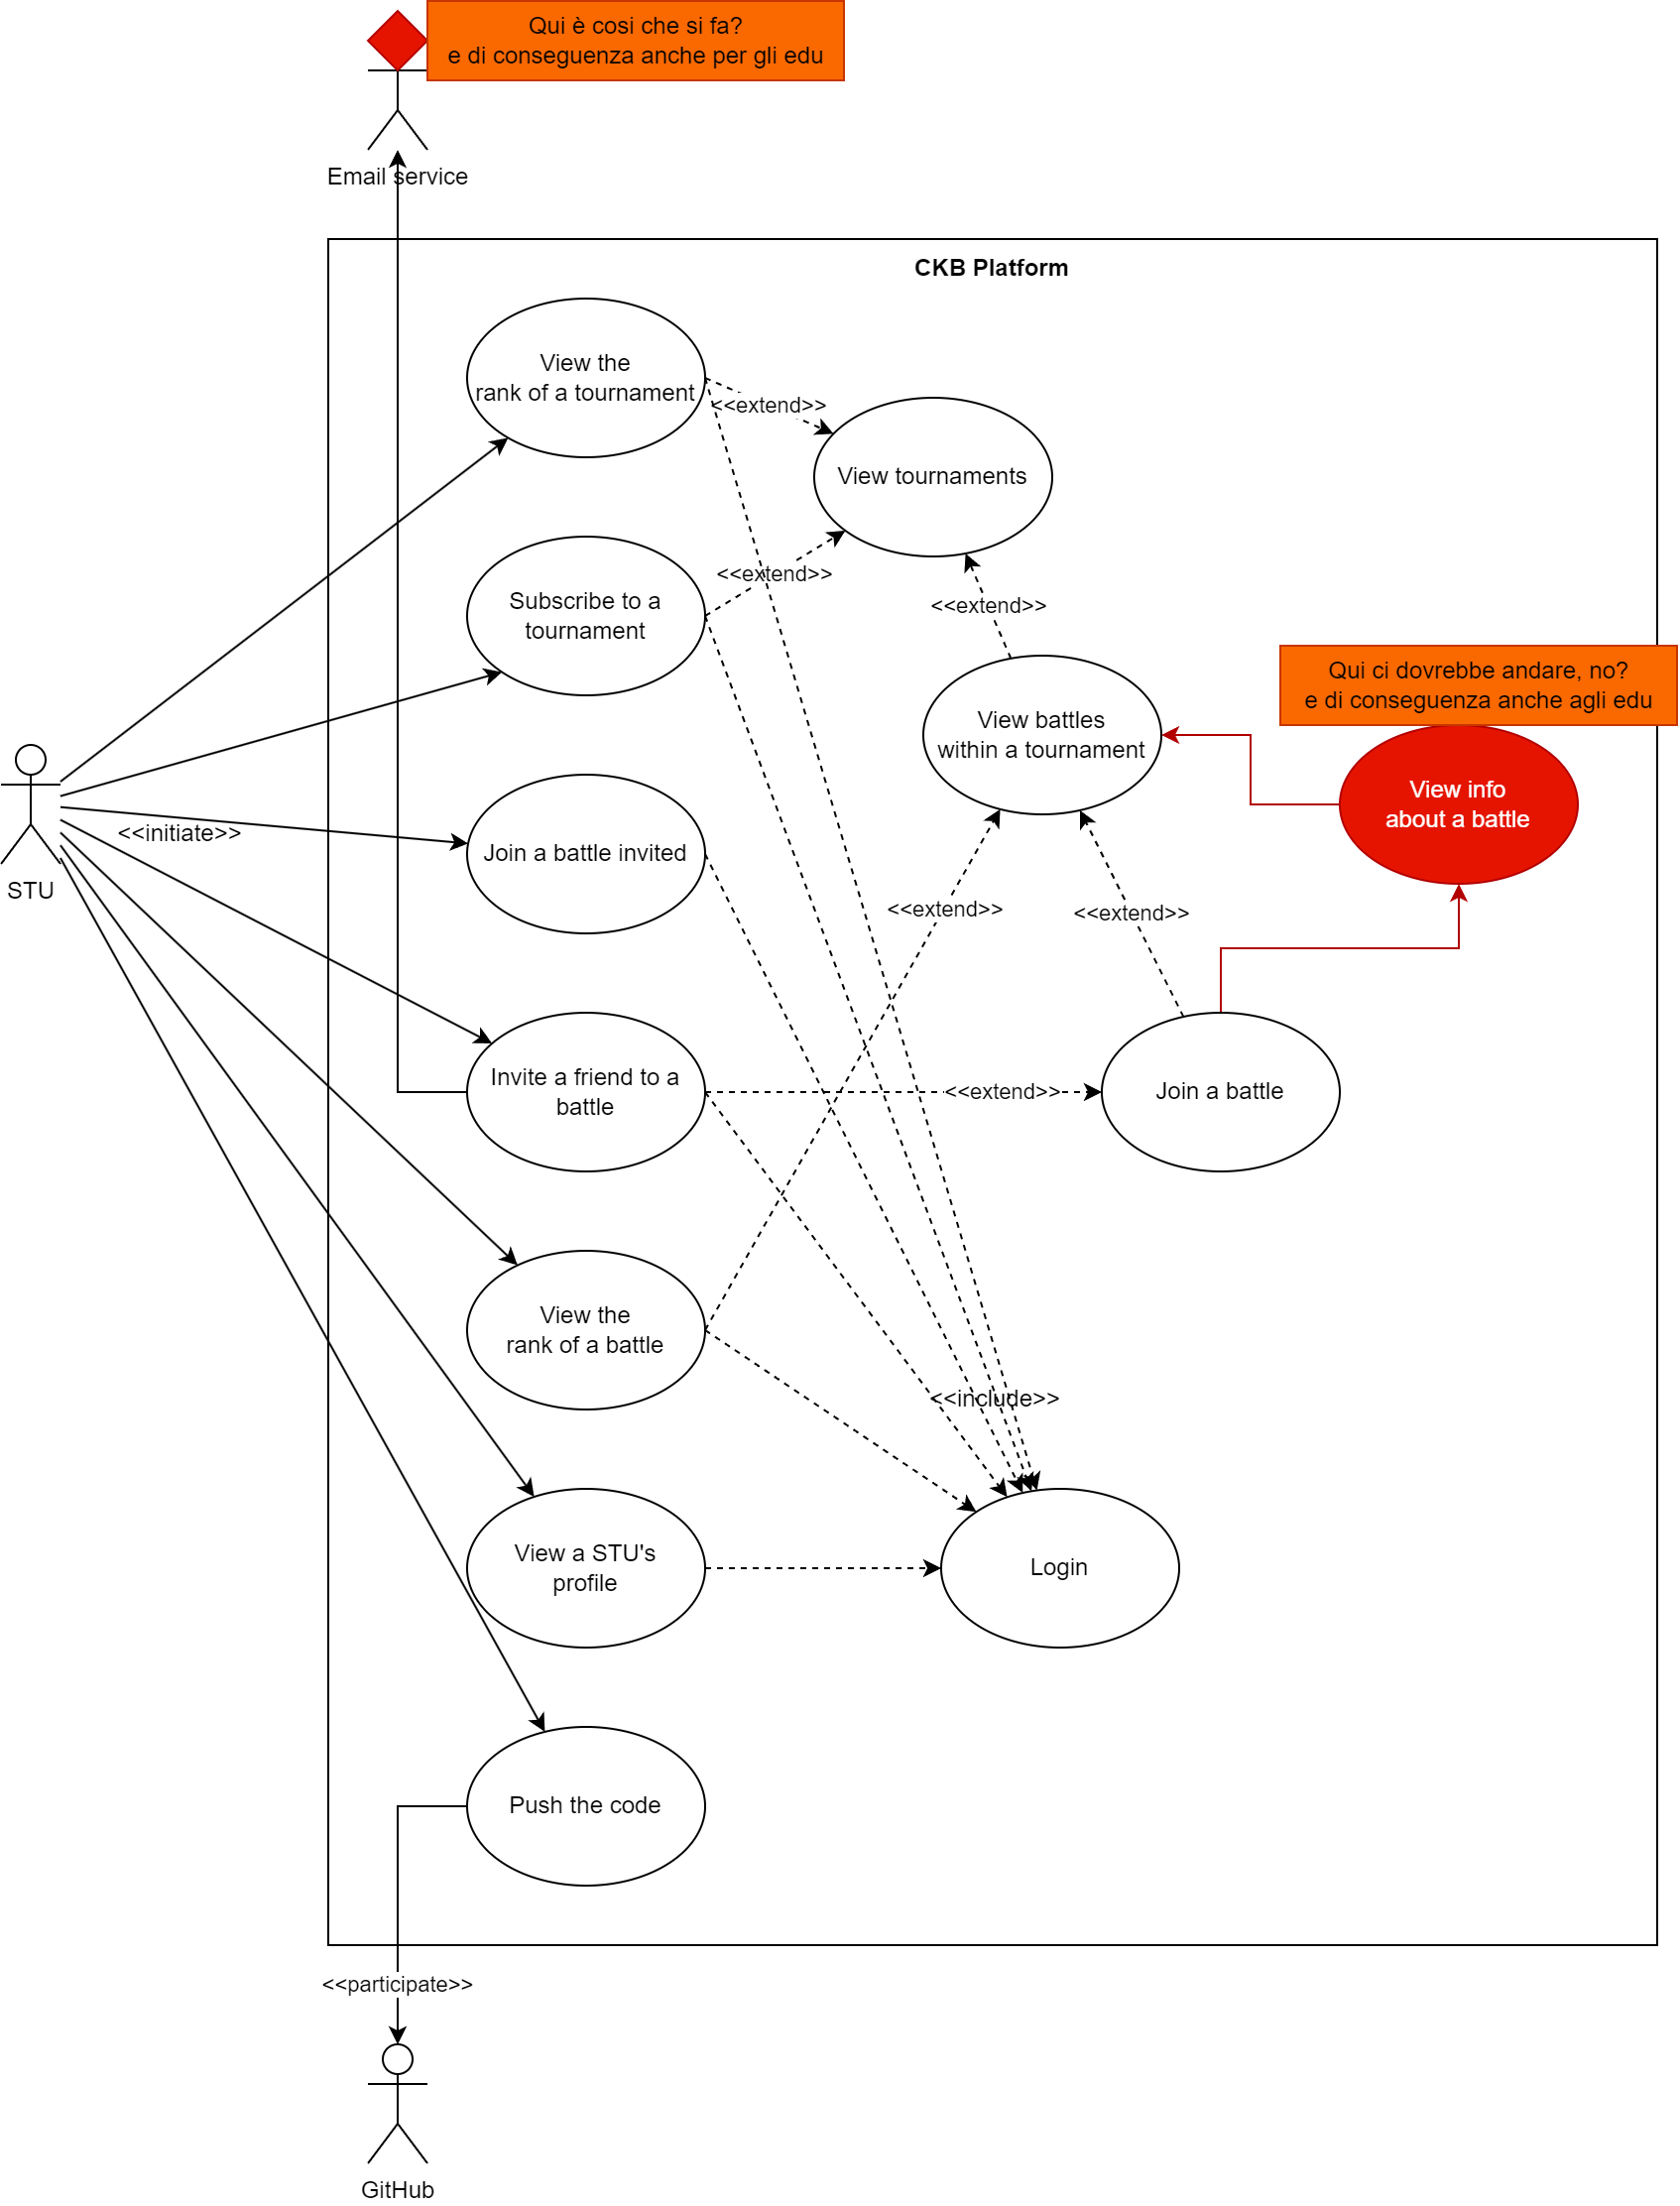
\includegraphics[width=0.8\textwidth]{images/sequence_diagrams/use_case_diagrams_STU.png}
    \caption{STU Use Case Diagram}
\end{figure}

\newpage

\subsection{Use cases Description}
The following use cases within the exception section do not contain, for the sake of enhancing readability and simplifying the sequence diagrams, these anomalies:
\begin{enumerate}
    \item Verification of the existence of the actor in the CKB system each time said actor undertakes an action.
    \item Verification of the possession of all requisite permissions by an actor before the execution of an action.
    \item Validation of submitted forms, to ensure the absence of data with illegal formats or empty fields.
    \item Assurance of the atomicity of each transaction, signifying its completion or abort.
\end{enumerate}
It is imperative to note that in the event of any anomalies related to these scenarios, appropriate error messages will be displayed on the user interface.

%% LAYOUT FOR THE TABLES:
% \begin{center}
%     \def\arraystretch{1.5}
%     \setlist[enumerate]{itemsep=.1pt}
%     \begin{tabular}{| m{2cm} | m{10cm}|}
%         \hline
%         Name                  &  \\ \hline
%         ID                    &  \\ \hline
%         Actors                &  \\ \hline
%         Entry \par conditions &  \\ \hline
%         Event \par flow            & \begin{enumerate}
%                                     \item
%                                     \item
%                                     \item
%                                     \item
%                                 \end{enumerate}                              \\ \hline
%         Exit \par conditions       &                                               \\ \hline
%         Exceptions            &                                               \\ \hline
%         Notes                &                                               \\ \hline   
%     \end{tabular}
% \end{center}

\begin{center}
    \def\arraystretch{1.5}
    \setlist[enumerate]{itemsep=.1pt}
    \begin{tabular}{| m{2cm} | m{10cm}|}
        \hline
        Name                  & Register                                                                                                                                \\ \hline
        ID                    & UC1 (Figure \ref{fig:uc1})                                                                                                              \\ \hline
        Actors                & EDU or STU                                                                                                                              \\ \hline
        Entry \par conditions & The actor is not registered and wants to create an account                                                                              \\ \hline
        Event \par flow       & \begin{enumerate}
                                    \item The actor enters the registration page
                                    \item The system shows the registration form
                                    \item The actor specifies whether is an educator or a student
                                    \item The actor fills out the form with truthful information
                                    \item The actor confirms the account creation
                                    \item The system creates an account concerning  the information inserted by the actor
                                \end{enumerate}                                                                                                                         \\ \hline
        Exit \par conditions  & The system successfully creates the account and shows the "Log in" page                                                                 \\ \hline
        Exceptions            & \begin{itemize}
                                    \item The actor inserts information (e.g. email) about an account that already exists: a human-readable message is displayed
                                \end{itemize}                                                                                                                           \\ \hline
    \end{tabular}
\end{center}

\begin{center}
    \def\arraystretch{1.5}
    \setlist[enumerate]{itemsep=.1pt}
    \begin{tabular}{| m{2cm} | m{10cm}|}
        \hline
        Name                  & Log in                                                                                                   \\ \hline
        ID                    & UC2 (Figure \ref{fig:uc2})                                                                               \\ \hline
        Actors                & EDU or STU                                                                                               \\ \hline
        Entry \par conditions & The actor is already subscribed to the CKB platform                                                      \\ \hline
        Event \par flow       & \begin{enumerate}
                                    \item The actor enters the "Log In" page
                                    \item The system shows the login form
                                    \item The actor fills the form with its credentials and submits it
                                    \item The system checks the credentials and logs the actor in
                                \end{enumerate}                                        \\ \hline
        Exit \par conditions  & The actor is logged in and the "Dashboard" page is displayed                                             \\ \hline
        Exceptions            & \begin{itemize}
                                    \item The actor inserts a wrong combination of username - password: a human-readable message is displayed
                                    \item The actor is not registered so the username does not exist: a human-readable message is displayed
                                \end{itemize} \\ \hline
    \end{tabular}
\end{center}

\begin{center}
    \def\arraystretch{1.5}
    \setlist[enumerate]{itemsep=.1pt}
    \begin{tabular}{| m{2cm} | m{10cm}|}
        \hline
        Name                  & Create tournament                                                                                                                       \\ \hline
        ID                    & UC3 (Figure \ref{fig:uc3})                                                                                                              \\ \hline
        Actors                & EDU and ESP                                                                                                                             \\ \hline
        Entry \par conditions & The actor is logged in as an EDU \textbf{and} it is in the "Dashboard" page                                                             \\ \hline
        Event \par flow       & \begin{enumerate}
                                    \item EDU clicks on the "Create new" button
                                    \item The system shows the "Create tournament" page with a form to be compiled
                                    \item EDU fills the form with the required information as Tournament name, STUs' registration window, and the optional list of badges
                                    \item EDU clicks on the "Create" button
                                    \item The system notifies all the registered STUs about the creation of a new tournament, by sending an email through ESP
                                    \item EDU is redirected to the "Dashboard" page showing the new tournament created
                                \end{enumerate}                                                                                                                         \\ \hline
        Exit \par conditions  & The system has created the new tournament                                                                                               \\ \hline
        Exceptions            & \begin{itemize}
                                    \item The EDU inserts a Tournament name already used for another tournament: a human-readable message is displayed
                                    \item The EDU specifies a deadline in the past: a human-readable message is displayed
                                \end{itemize}                                                                                                                           \\ \hline
    \end{tabular}
\end{center}

\begin{center}
    \def\arraystretch{1.5}
    \setlist[enumerate]{itemsep=.1pt}
    \begin{tabular}{| m{2cm} | m{10cm}|}
        \hline
        Name                  & Create Battle                                                                                                                                                                       \\ \hline
        ID                    & UC4 (Figure \ref{fig:uc4})                                                                                                                                                          \\ \hline
        Actors                & EDU and ESP                                                                                                                                                                                \\ \hline
        Entry \par conditions & The actor is logged in as an EDU \textbf{and} it is in the "Dashboard" page \textbf{and} it has the permission to create battles inside a specific tournament                       \\ \hline
        Event \par flow       & \begin{enumerate}
                                    \item The EDU clicks on the tournament in which it wants to create a new battle
                                    \item The system shows the "Tournament View" page with the "Create new battle" button
                                    \item The EDU clicks the "Create new battle" button
                                    \item The system shows the "Battle creation" page with a form to be compiled 
                                    \item The EDU fills the form with the details about the battle (e.g. battle name, code language, deadlines) and uploads the Code Kata
                                    \item The system checks if all fields are correctly filled and then creates the battle
                                \end{enumerate}                                                                                                                                                                     \\ \hline
        Exit \par conditions  & All STU subscribed to the tournament in which the battle is created get notified through ESP, that a new battle is available                                                        \\ \hline
        Exceptions            & \begin{itemize}
                                    \item The EDU does not have enough permissions for the selected tournament: the system does not show the "Create new battle" button
                                \end{itemize}                                                                                                                                                                       \\ \hline
    \end{tabular}
\end{center}

\begin{center}
    \def\arraystretch{1.5}
    \setlist[enumerate]{itemsep=.1pt}
    \begin{tabular}{| m{2cm} | m{10cm}|}
        \hline
        Name                  & Share permission                                                                                                        \\ \hline
        ID                    & UC5 (Figure \ref{fig:uc5})                                                                                              \\ \hline
        Actors                & EDU                                                                                                                     \\ \hline
        Entry \par conditions & The actor is logged in as an EDU \textbf{and} it is in the "Dashboard" page \textbf{and} a tournament is in progress    \\ \hline
        Event \par flow       & \begin{enumerate}
                                    \item The EDU selects a tournament it has created
                                    \item The system shows the "Tournament View" page
                                    \item The EDU clicks on the "Share permission" button
                                    \item The system shows the list of all the EDUs subscribed to the CKB platform
                                    \item The EDU searches the EDU(s) to which it wants to share the permission
                                    \item The user adds an EDU to the tournament by clicking the "Add" button
                                \end{enumerate}                                                                                                         \\ \hline
        Exit \par conditions  & The other EDU(s) can now create battles within that tournament                                                          \\ \hline
        Exceptions            & \begin{itemize}
                                    \item The actor opens a tournament that does not exist: a human-readable message is displayed
                                    \item The actor searches for an EDU that does not exist in the system: a human-readable message is displayed
                                    \item The actor adds an EDU already part of the tournament: a human-readable message is displayed
                                \end{itemize}                                                                                                           \\ \hline
        Note                  & To make the research of a specific EDU easier, the system provides a search bar                                         \\ \hline
    \end{tabular}
\end{center}

\begin{center}
    \def\arraystretch{1.5}
    \setlist[enumerate]{itemsep=.1pt}
    \begin{tabular}{| m{2cm} | m{10cm}|}
        \hline
        Name                  & Join a tournament                                                                                           \\ \hline
        ID                    & UC6 (Figure \ref{fig:uc6})                                                                                  \\ \hline
        Actors                & STU                                                                                                         \\ \hline
        Entry \par conditions & The actor is logged in as a STU \textbf{and} it has received an e-mail from about a new tournament created  \\ \hline
        Event \par flow       & \begin{enumerate}
                                    \item STU opens the e-mail and clicks on the link attached to be redirected to the tournament
                                    \item The system shows the "Tournament View" page
                                    \item STU clicks on the "Join Tournament" button
                                    \item The system processes the request and confirms the enrollment
                                \end{enumerate}                                                                                             \\ \hline
        Exit \par conditions  & STU is now part of that tournament                                                                          \\ \hline
        Exceptions            & \begin{itemize}
                                    \item The actor opens a tournament that does not exist: a human-readable message is displayed
                                    \item The tournament registration window is expired: a human-readable message is displayed
                                    \item The STU is already part of the tournament: a human-readable message is displayed
                                \end{itemize}                                                                                               \\ \hline
    \end{tabular}
\end{center}

\begin{center}
    \def\arraystretch{1.5}
    \setlist[enumerate]{itemsep=.1pt}
    \begin{tabular}{| m{2cm} | m{10cm}|}
        \hline
        Name                  & Join a Battle                                                                                                                                                                       \\ \hline
        ID                    & UC7 (Figure \ref{fig:uc7})                                                                                                                                                          \\ \hline
        Actors                & STU and ESP                                                                                                                                                                         \\ \hline
        Entry \par conditions & The actor is logged in as a STU \textbf{and} a tournament is in progress \textbf{and} the STU is subscribed to that tournament                                                      \\ \hline
        Event \par flow       & \begin{enumerate}
                                    \item The STU clicks on the tournament in which it wants to battle
                                    \item The system shows the "Tournament View" page with a list of battles
                                    \item The STU clicks on the battle it wants to join
                                    \item The system shows the "Battle View" page with all the information about it, if the subscribing deadline has not expired yet, the system shows the "Join Battle" button
                                    \item The STU clicks on the "Join Battle" button to enter the battle
                                    \item The system displays a form to create a team and invite other members
                                    \item The STU, if wants or must invite friends to be part of its team, inserts their emails and then presses the "Join" button
                                    \item The system sends an email to each invited member
                                \end{enumerate}                                                                                                                                                                     \\ \hline
        Exit \par conditions  & The system subscribes the STU to the battle that now waits for the reply of other STUs or can invite other mates to the team                                                         \\ \hline
        Exceptions            & \begin{itemize}
                                    \item The STU wants to invite a number of mates greater or less than the boundaries imposed: a human-readable message is displayed
                                    \item The deadline expires and the team does not satisfy the constraint for the minimum team participants: the team is not enrolled in the battle
                                    \item The emails inserted are not subscribed to the tournament: a human-readable message is displayed
                                \end{itemize}                                                                                                                                                                       \\ \hline
        Note                  & \begin{itemize}
                                    \item To make the research of a specific STU easier, the system provides a search bar
                                    \item The system offers the possibility to invite new members to the team and let other STUs join it, iff boundaries constraint are respected            
                                \end{itemize}                                                                                                                                                                       \\ \hline
    \end{tabular}
\end{center}

\begin{center}
    \def\arraystretch{1.5}
    \setlist[enumerate]{itemsep=.1pt}
    \begin{tabular}{| m{2cm} | m{10cm}|}
        \hline
        Name                  & Join a team - when already in the battle                                                                                                                                                                                                                                                            \\ \hline
        ID                    & UC8.1 (Figure \ref{fig:uc8})                                                                                                                                                                                                                                                                        \\ \hline
        Actors                & STU                                                                                                                                                                                                                                                                                                 \\ \hline
        Entry \par conditions & STU is registered in CKB platform \textbf{and} is enrolled in a tournament \textbf{and} has received an email notification from the system inviting it to join a team for an upcoming battle within the context of the enrolled tournament \textbf{and} it has already joined that battle alone     \\ \hline
        Event \par flow       & \begin{enumerate}
                                    \item User opens the e-mail and clicks on the link attached to be redirected to the system
                                    \item The system shows the "Dashboard" page with the invitation if the join window for the battle is still open
                                    \item User decides to Accept or Decline the invite
                                    \begin{itemize}
                                        \item User clicks the "Accept" button
                                    \end{itemize}
                                        \begin{enumerate}
                                            \item The system adds the STU to the team
                                            \item User now is part of that team in the battle
                                        \end{enumerate}
                                    \begin{itemize}
                                        \item User clicks the "Decline" button
                                    \end{itemize}
                                        \begin{enumerate}
                                            \item The system deletes the notification from its "Dashboard" page
                                            \item The system notifies the STU that sent the invite of the decision and allows it to invite a new STU
                                        \end{enumerate}
                                \end{enumerate}                                                                                                                                                                                                                                                                                     \\ \hline
        Exit \par conditions  & STU participates in the battle, depending on its choice, alone or in a team of more than one STU                                                                                                                                                                                                    \\ \hline
        Exceptions            & \begin{itemize}
                                    \item STU ignores the invite received: STU participates alone and at the end of the registration window, for that specific battle, all the invites related are canceled from the "Dashboard" page
                                    \item STU received multiple invitations for the same battle, but from different teams: after one invite is accepted all the others are canceled in its "Dashboard" page
                                    \item STUs already part of a team can not be selected to be in a different team
                                \end{itemize}                                                                                                                                                                                                                                                                                       \\ \hline
    \end{tabular}
\end{center}

\begin{center}
    \def\arraystretch{1.5}
    \setlist[enumerate]{itemsep=.1pt}
    \begin{tabular}{| m{2cm} | m{10cm}|}
        \hline
        Name                  & Join a team - when not in the battle yet                                                                                                                                                                                                        \\ \hline
        ID                    & UC8.2 (Figure \ref{fig:uc8})                                                                                                                                                                                                                    \\ \hline
        Actors                & STU                                                                                                                                                                                                                                             \\ \hline
        Entry \par conditions & STU is registered in CKB platform \textbf{and} is enrolled in a tournament \textbf{and} has received an email notification from the system inviting it to join a team for an upcoming battle within the context of the enrolled tournament      \\ \hline
        Event \par flow       & \begin{enumerate}
                                    \item User opens the e-mail and clicks on the link attached to be redirected to the system
                                    \item The system shows the "Dashboard" page with the invitation if the join windows for the battle is still open
                                    \item User decides to Accept or Decline the invite
                                    \begin{itemize}
                                        \item User click the "Accept" button
                                    \end{itemize}
                                        \begin{enumerate}
                                            \item The system enrolls the STU to the battle and then adds it to the team that sent the invite
                                            \item User is part of the battle and it competes in it with a team
                                        \end{enumerate}
                                    \begin{itemize}
                                        \item User clicks the "Decline" button
                                    \end{itemize}
                                        \begin{enumerate}
                                            \item The system deletes the notification from its "Dashboard" page
                                            \item The system notifies the STU that sent the invite of the decision and allows it to invite a new STU
                                        \end{enumerate}
                                \end{enumerate}                                                                                                                                                                                                                                 \\ \hline
        Exit \par conditions  & STU is part of the battle and the team if it accepts the invite, else is not part of none of that                                                                                                                                               \\ \hline
        Exceptions            & \begin{itemize}                                    
                                    \item STU ignores the invite received: STU is neither part of the battle nor the team and at the end of the registration window, for that specific battle, all the related invites are canceled from the "Dashboard" page
                                    \item STU received multiple invitations for the same battle, but from different teams: after one invite is accepted all the others are canceled in its "Dashboard" page
                                    \item STUs already part of a team can not be selected to be in a different team
                                \end{itemize}                                                                                                                                                                                                                                   \\ \hline
    \end{tabular}
\end{center}

\begin{center}
    \def\arraystretch{1.5}
    \setlist[enumerate]{itemsep=.1pt}
    \begin{tabular}{| m{2cm} | m{10cm}|}
        \hline
        Name                  & Manual evaluation                                                                                                                                                                           \\ \hline
        ID                    & UC9 (Figure \ref{fig:uc9})                                                                                                                                                                  \\ \hline
        Actors                & EDU ans ESP                                                                                                                                                                                 \\ \hline
        Entry \par conditions & The actor is logged in as an EDU \textbf{and} it is on the "Tournament View" where at least a battle's deadline has expired \textbf{and} that battle has the "manual evaluation" enabled    \\ \hline
        Event \par flow       & \begin{enumerate}
                                    \item The EDU selects a battle it has created
                                    \item The system shows the "Battle View" page, which has a list of all the teams that have submitted their work within the deadline
                                    \item One by one, the EDU selects a team and the system shows the team's code
                                    \item The EDU evaluates the code and assigns a score in the range [0, 100]
                                    \item The EDU clicks on the "Submit" button
                                    \item The system updates the battle score of the team
                                    \item When all the teams are evaluated, the EDU clicks on the "Close battle" button
                                \end{enumerate}                                                                                                                                                                             \\ \hline
        Exit \par conditions  & All participants in the battle get notified through ESP, that the final score is available                                                                                                  \\ \hline
        Exceptions            & \begin{itemize}
                                    \item The EDU does not evaluate the code of a team and clicks on the "Submit" button: a human-readable message is displayed
                                    \item The EDU assigns a score that is not in the range [0, 100]: a human-readable message is displayed
                                    \item The EDU wants to change the score assigned to a team: the system lets the EDU change the score and then it updates the battle score of the team
                                \end{itemize}                                                                                                                                                                               \\ \hline
        Note                  & The system offers the possibility to stop the evaluation process, it saves the scores assigned to the teams and the evaluation process can be resumed later                                 \\ \hline
    \end{tabular}
\end{center}

\begin{center}
    \def\arraystretch{1.5}
    \setlist[enumerate]{itemsep=.1pt}
    \begin{tabular}{| m{2cm} | m{10cm}|}
        \hline
        Name                  & Create new badge                                                                                                                        \\ \hline
        ID                    & UC10 (Figure \ref{fig:uc10})                                                                                                            \\ \hline
        Actors                & EDU                                                                                                                                     \\ \hline
        Entry \par conditions & The user is logged in as EDU \textbf{and} it is in the "Dashboard" page                                                                 \\ \hline
        Event \par flow       & \begin{enumerate}
                                    \item EDU clicks on the "Badges" button
                                    \item The system shows the "Create badge" page with a form to be compiled
                                    \item EDU fills the form with the required information as a title and rule that STU must fulfill to obtain that specific badge
                                    \item EDU clicks on the "Create" button
                                    \item The system redirects the EDU to the "Dashboard" page
                                \end{enumerate}                                                                                                                         \\ \hline
        Exit \par conditions  & The systems create the new badge and now available whenever EDUs in CKB create tournaments                                              \\ \hline
        Exceptions            & \textit{None}                                                                                                                           \\ \hline
    \end{tabular}
\end{center}

\begin{center}
    \def\arraystretch{1.5}
    \setlist[enumerate]{itemsep=.1pt}
    \begin{tabular}{| m{2cm} | m{10cm}|}
        \hline
        Name                  & Close tournament                                                                                                                                \\ \hline
        ID                    & UC11 (Figure \ref{fig:uc11})                                                                                                                    \\ \hline
        Actors                & EDU and ESP                                                                                                                                     \\ \hline
        Entry \par conditions & The actor is logged in as an EDU \textbf{and} it has all the authorization in the tournament \textbf{and} it is in the "Tournament View" page   \\ \hline
        Event \par flow       & \begin{enumerate}
                                    \item The EDU clicks on the "Close tournament" button
                                    \item The system shows a confirmation message
                                    \item The EDU clicks on the "Confirm" button
                                    \item The system closes the tournament and elaborates the final tournament rank
                                \end{enumerate}                                                                                                                                 \\ \hline
        Exit \par conditions  & All the STUs enrolled in the tournament get notified through ESP and can check the tournament final ranking                                     \\ \hline
        Exceptions            & \begin{itemize}
                                    \item The EDU clicks on the "Cancel" button: the system closes the message and shows normally the tournament page
                                    \item The tournament is already closed: a human-readable message is displayed
                                \end{itemize}                                                                                                                                   \\ \hline
    \end{tabular}
\end{center}

\begin{center}
    \def\arraystretch{1.5}
    \setlist[enumerate]{itemsep=.1pt}
    \begin{tabular}{| m{2cm} | m{10cm}|}
        \hline
        Name                  & View battle rank                                                                                                                                            \\ \hline
        ID                    & UC12 (Figure \ref{fig:uc12})                                                                                                                                \\ \hline
        Actors                & EDU and STU                                                                                                                                                 \\ \hline
        Entry \par conditions & The actor is logged in as an EDU or a STU \textbf{and} it is in the "Tournament View" page of the tournament containing the battle is looking forking       \\ \hline
        Event \par flow       & \begin{enumerate}
                                    \item The actor searches through battles
                                    \item The actor clicks on the chosen battle
                                    \item The system shows the rank of that battle next to the battle list
                                \end{enumerate}                                                                                                                                             \\ \hline
        Exit \par conditions  & The actor can see the rank of the battle it was looking for                                                                                                 \\ \hline
        Exceptions            & \textit{None}                                                                                                                                               \\ \hline
        Note                  & If the battle is not started yet, the system will show an empty rank                                                                                        \\ \hline
    \end{tabular}
\end{center}

\begin{center}
    \def\arraystretch{1.5}
    \setlist[enumerate]{itemsep=.1pt}
    \begin{tabular}{| m{2cm} | m{10cm}|}
        \hline
        Name                  & View tournament rank                                                                                \\ \hline
        ID                    & UC13 (Figure \ref{fig:uc13})                                                                        \\ \hline
        Actors                & EDU or STU                                                                                          \\ \hline
        Entry \par conditions & The actor is logged in as an EDU or a STU \textbf{and} it is in the "Dashboard" page                \\ \hline
        Event \par flow       & \begin{enumerate}
                                    \item The system shows the list of all the tournaments
                                    \item The actor selects a tournament, either ongoing or closed
                                    \item The system shows the "Tournament View" page
                                \end{enumerate}                                                                                     \\ \hline
        Exit \par conditions  & The actor can now see the tournament rank                                                           \\ \hline
        Exceptions            & \textit{None}                                                                                       \\ \hline
        Notes                 & The "Tournament View" page shows both the rank and the list of battles within it, ongoing or ended  \\ \hline
    \end{tabular}
\end{center}

\begin{center}
    \def\arraystretch{1.5}
    \setlist[enumerate]{itemsep=.1pt}
    \begin{tabular}{| m{2cm} | m{10cm}|}
        \hline
        Name                  & View STU's profile                                                                                                      \\ \hline
        ID                    & UC14 (Figure \ref{fig:uc14})                                                                                            \\ \hline
        Actors                & EDU or STU                                                                                                              \\ \hline
        Entry \par conditions & The actor is logged in as an EDU or a STU                                                                               \\ \hline
        Event \par flow       & \begin{enumerate}
                                    \item The actor clicks on a STU username
                                    \item The system redirects the actor to the "Profile View" page of the STU with that username
                                \end{enumerate}                                                                                                         \\ \hline
        Exit \par conditions  & The user sees the profile of the STU, it can visualize gained badges and the list of the tournament it is enrolled in    \\ \hline
        Exceptions            & \begin{enumerate}
                                    \item There is no STU with the username specified
                                \end{enumerate}                                                                                                         \\ \hline
    \end{tabular}
\end{center}

\begin{center}
    \def\arraystretch{1.5}
    \setlist[enumerate]{itemsep=.1pt}
    \begin{tabular}{| m{2cm} | m{10cm}|}
        \hline
        Name                  & View tournaments                                                                                                                \\ \hline
        ID                    & UC15.1 (Figure \ref{fig:uc15.1})                                                                                                  \\ \hline
        Actors                & EDU                                                                                                                             \\ \hline
        Entry \par conditions & The actor is logged in as an EDU \textbf{and} it is in the "Dashboard" page                                                     \\ \hline
        Event \par flow       & \begin{enumerate}
                                    \item The system, in the "Dashboard" page, shows the list of all tournaments created by the EDU
                                    \item The EDU can select a tournament, either ongoing or closed
                                    \item The system shows the "Tournament View" page with the list of its ongoing or closed battles
                                \end{enumerate}                                                                                                                 
                                \textbf{Alternatively:}
                                \begin{enumerate}
                                    \item The EDU, in the "Dashboard" page, clicks on the "Show all" button
                                    \item The EDU type in the search bar the name of a tournament it is looking for
                                    \item The system shows the matching result 
                                    \item The EDU can select the resulting tournament, either ongoing or closed
                                    \item The system shows the "Tournament View" page with the list of its ongoing or closed battles
                                \end{enumerate}                                                                                                                 \\ \hline
        Exit \par conditions  & The EDU see the "Tournament View" page and can take actions in it                                                               \\ \hline
        Exceptions            & \begin{enumerate}
                                    \item The EDU type, in the search bar, a tournament name that does not exist: a human-readable message is displayed
                                \end{enumerate}                                                                                                                 \\ \hline
    \end{tabular}
\end{center}


\begin{center}
    \def\arraystretch{1.5}
    \setlist[enumerate]{itemsep=.1pt}
    \begin{tabular}{| m{2cm} | m{10cm}|}
        \hline
        Name                  & View tournaments                                                                                                                                                                \\ \hline
        ID                    & UC15.2 (Figure \ref{fig:uc15.2})                                                                                                                                                  \\ \hline
        Actors                & STU                                                                                                                                                                             \\ \hline
        Entry \par conditions & The actor is logged in as a STU \textbf{and} it is in the "Dashboard" page                                                                                                      \\ \hline
        Event \par flow       & \begin{enumerate}
                                    \item The system, in the "Dashboard" page, shows the list of all the tournaments to which the STU is subscribed
                                    \item The STU can select a tournament, either ongoing or closed
                                    \item The system shows the "Tournament View" page with the list of its ongoing or closed battles
                                \end{enumerate}
                                \textbf{Alternatively:}
                                \begin{enumerate}
                                    \item The STU, in the "Dashboard" page, clicks on the "Show all" button
                                    \item The STU type in the search bar the name of a tournament it is looking for
                                    \item The system shows the matching result 
                                    \item The STU can select the resulting tournament, either ongoing or closed
                                    \item The system shows the "Tournament View" page with the list of its ongoing or closed battles
                                \end{enumerate}                                                                                                                                                                 \\ \hline
        Exit \par conditions  & The STU see the "Tournament View" page and can take actions in it                                                                                                               \\ \hline
        Exceptions            & \begin{enumerate}
                                    \item The STU type, in the search bar, a tournament name that does not exist: the system suggests other tournaments showing their names and the subscribing deadlines
                                \end{enumerate}                                                                                                                                                                 \\ \hline
        Notes                 & In the "Dashboard" page are shown both suggested tournaments and tournaments to which the STU is subscribed                                                                     \\ \hline
    \end{tabular}
\end{center}


\begin{center}
    \def\arraystretch{1.5}
    \setlist[enumerate]{itemsep=.1pt}
    \begin{tabular}{| m{2cm} | m{10cm}|}
        \hline
        Name                  & View battles in tournament                                                                  \\ \hline
        ID                    & UC16 (Figure \ref{fig:uc16})                                                                \\ \hline
        Actors                & EDU or STU                                                                                  \\ \hline
        Entry \par conditions & The actor is logged as an EDU or a STU \textbf{and} it is in the "Dashboard" page           \\ \hline
        Event \par flow       & \begin{enumerate}
                                    \item The actor selects a tournament
                                    \item The system shows the "Tournament View" page
                                \end{enumerate}                                                                             \\ \hline
        Exit \par conditions  & The actor can see the list of all battles within that tournament                            \\ \hline
        Exceptions            & \textit{None}                                                                               \\ \hline
        Notes                 & The tournament page shows both the rank and the list of battles within it, ongoing or ended \\ \hline
    \end{tabular}
\end{center}

\begin{center}
    \def\arraystretch{1.5}
    \setlist[enumerate]{itemsep=.1pt}
    \begin{tabular}{| m{2cm} | m{10cm}|}
        \hline
        Name                  & Push commit and score updating                                                                                                                                          \\ \hline
        ID                    & UC17 (Figure \ref{fig:uc17})                                                                                                                                            \\ \hline
        Actors                & STU and GitHub API                                                                                                                                                      \\ \hline
        Entry \par conditions & STU is subscribed to the battle \textbf{and} the registration deadline for a battle has expired \textbf{and} the battle is in progress and not ended yet                \\ \hline
        Event \par flow       & \begin{enumerate}
                                    \item STU pushes changes to its GitHub repository
                                    \item GitHub actions inform the CKB platform's API of a new push has been performed by STU
                                    \item The system pulls the latest sources and analyzes them
                                    \item The system runs the tests on the corresponding executables
                                    \item The system computes and updates the battle score of the team corresponding to STU
                                \end{enumerate}                                                                                                                                                         \\ \hline
        Exit \par conditions  & The STU's team can see the updated score                                                                                                                                \\ \hline
        Exceptions            & \textit{None}                                                                                                                                                           \\ \hline
        Notes                 & We assumed, in the Domain Assumptions section, that the STU set properly the GitHub repository and actions, so, by the side of the platform, nothing could go wrong     \\ \hline
    \end{tabular}
\end{center}

\begin{center}
    \def\arraystretch{1.5}
    \setlist[enumerate]{itemsep=.1pt}
    \begin{tabular}{| m{2cm} | m{10cm}|}
        \hline
        Name                  & Repository creation                                                                                                                         \\ \hline
        ID                    & UC18 (Figure \ref{fig:uc18})                                                                                                                \\ \hline
        Actors                & STU, GitHub API and ESP                                                                                                                     \\ \hline
        Entry \par conditions & The actor is logged in as a STU \textbf{and} it is subscribed to a battle \textbf{and} the registration deadline for that battle is expired \\ \hline
        Event \par flow       & \begin{enumerate}
                                    \item The system creates a GitHub repository for the battle through the GitHub API
                                    \item The system sends an email to all STUs subscribed to the battle with the link to the GitHub repository
                                    \item The STU clicks on the link and is redirected to the GitHub repository
                                \end{enumerate}                                                                                                                             \\ \hline
        Exit \par conditions  & The STU its team can start working on the Code Kata, just after forking the repository and setting up an automated workflow                 \\ \hline
        Exceptions            & \textit{None}                                                                                                                               \\ \hline
        Notes                 & Only one student per team receives the GitHub repository link via mail, moreover, the correct functioning of the API is assumed              \\ \hline
    \end{tabular}
\end{center}

\subsection{Use cases Sequence Diagrams}
\begin{figure}[H]
    \centering
    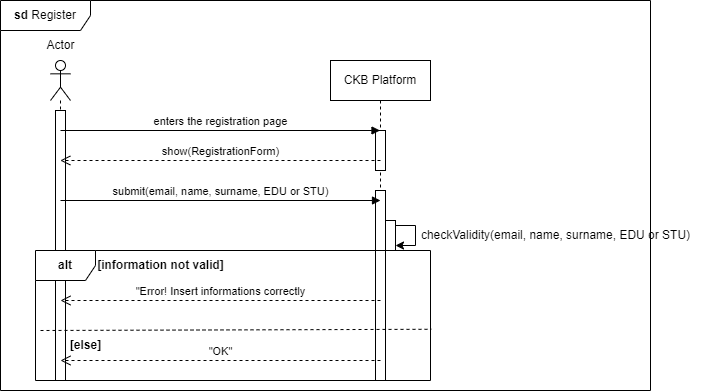
\includegraphics[width=1\textwidth]{images/sequence_diagrams/ClassDiagram-UC1 -SequenceDiagram.png}
    \caption{Register Use Case}
    \label{fig:uc1}
\end{figure}
\begin{figure}[H]
    \centering
    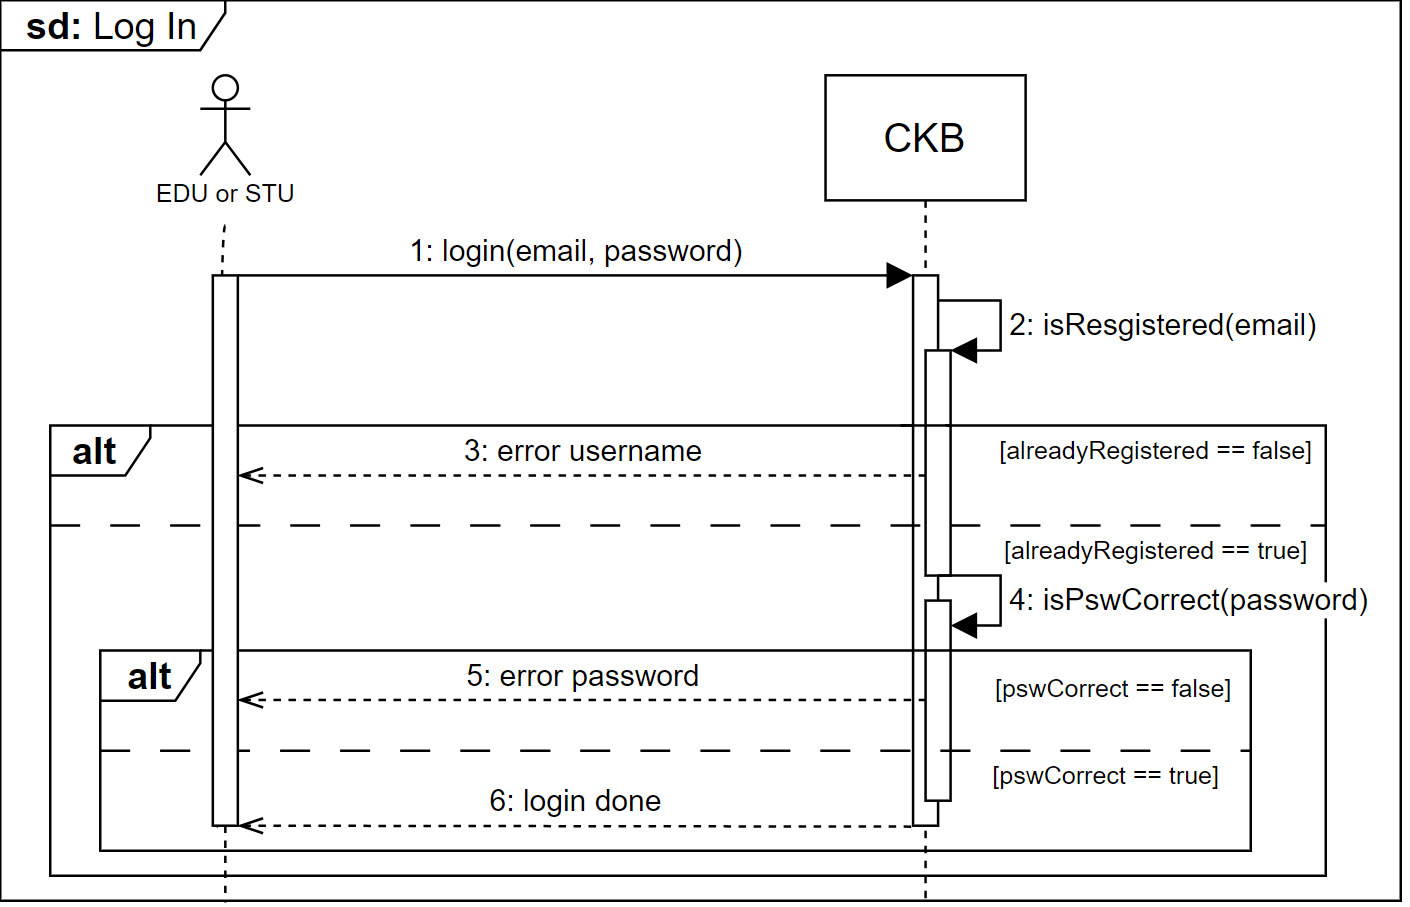
\includegraphics[width=1\textwidth]{images/sequence_diagrams/.png/Log_In - UC2.png}
    \caption{Log In Use Case}
    \label{fig:uc2}
\end{figure}
\begin{figure}[H]
    \centering
    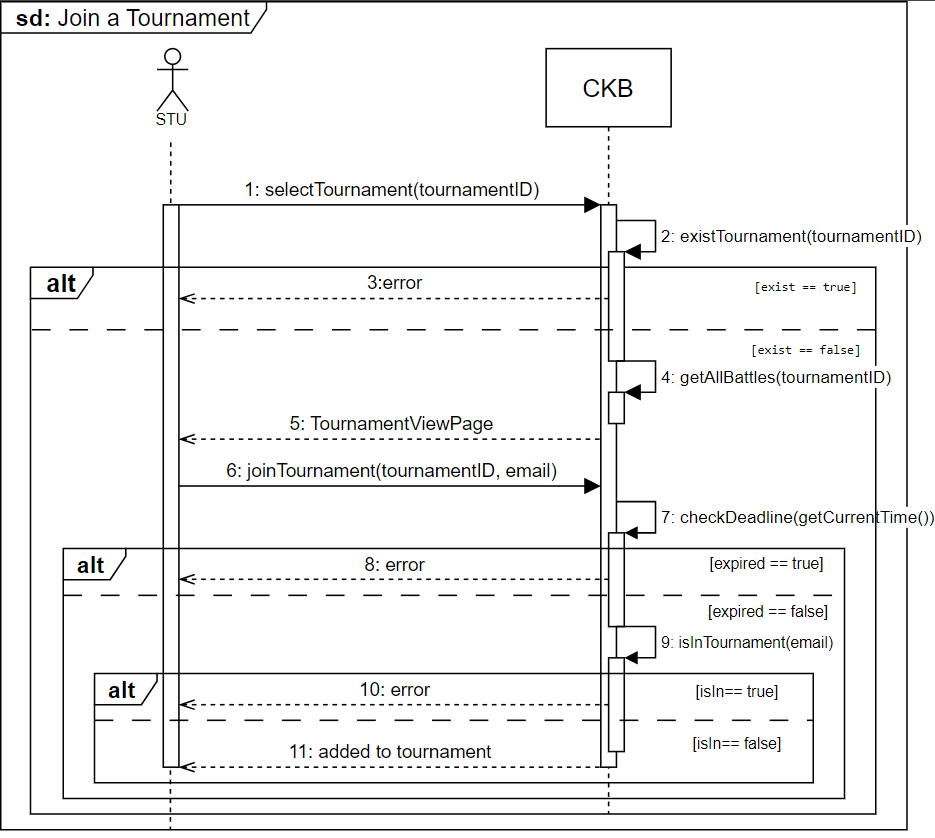
\includegraphics[width=1\textwidth]{images/sequence_diagrams/.png/Create_Tournament - UC3.png}
    \caption{Create a Tournament Use Case}
    \label{fig:uc3}
\end{figure}
\begin{figure}[H]
    \centering
    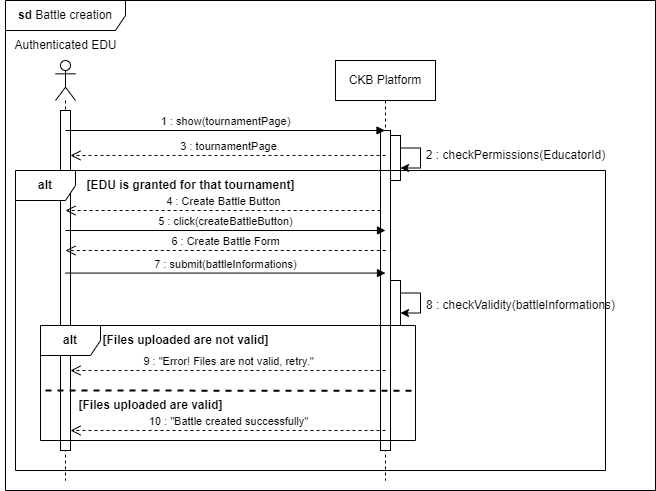
\includegraphics[width=1\textwidth]{images/sequence_diagrams/ClassDiagram-UC4- SequenceDiagram.png}
    \caption{Battle creation Use Case}
    \label{fig:uc4}
\end{figure}
\begin{figure}[H]
    \centering
    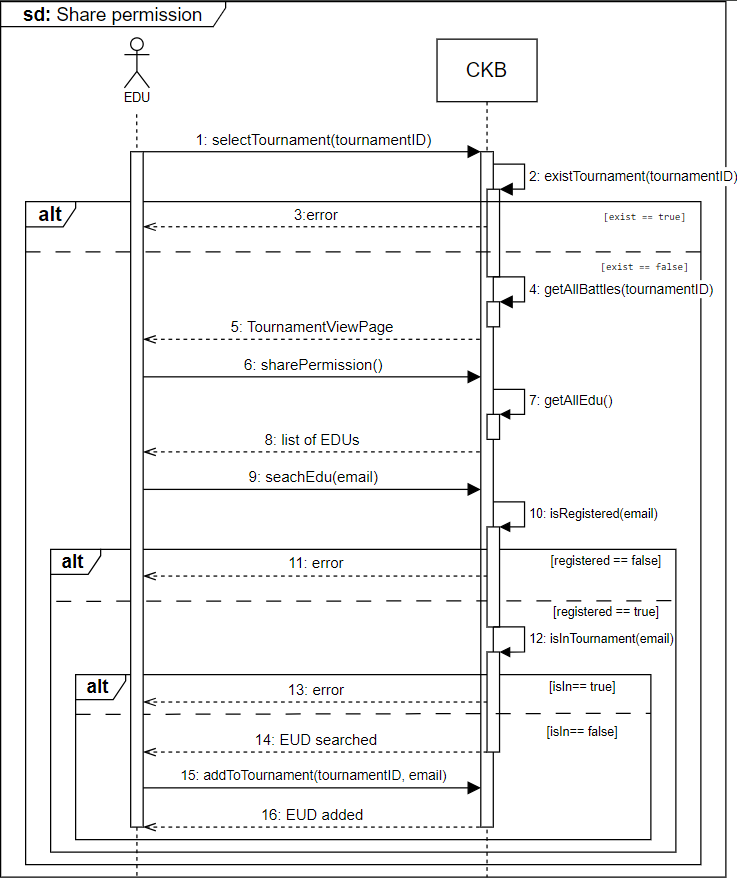
\includegraphics[width=1\textwidth]{images/sequence_diagrams/.png/Share_Permission - UC5.png}
    \caption{Share permission Use Case}
    \label{fig:uc5}
\end{figure}
\begin{figure}[H]
    \centering
    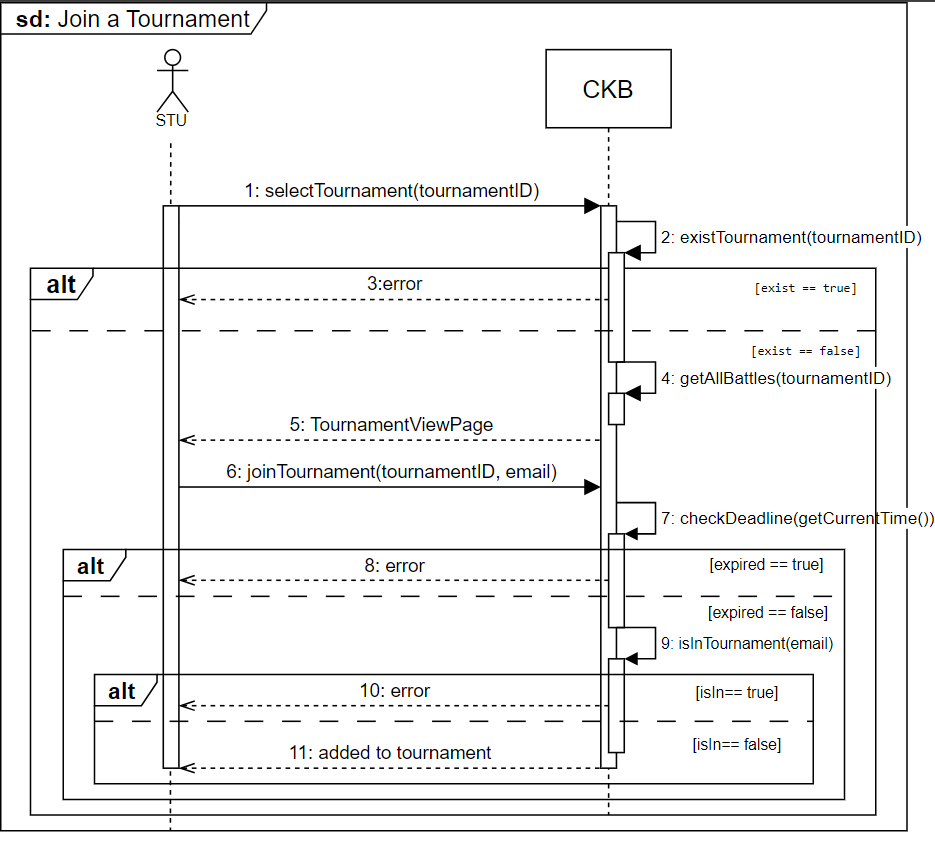
\includegraphics[width=1\textwidth]{images/sequence_diagrams/.png/Join_Tournament - UC6.png}
    \caption{Join a tournament Use Case}
    \label{fig:uc6}
\end{figure}
\begin{figure}[H]
    \centering
    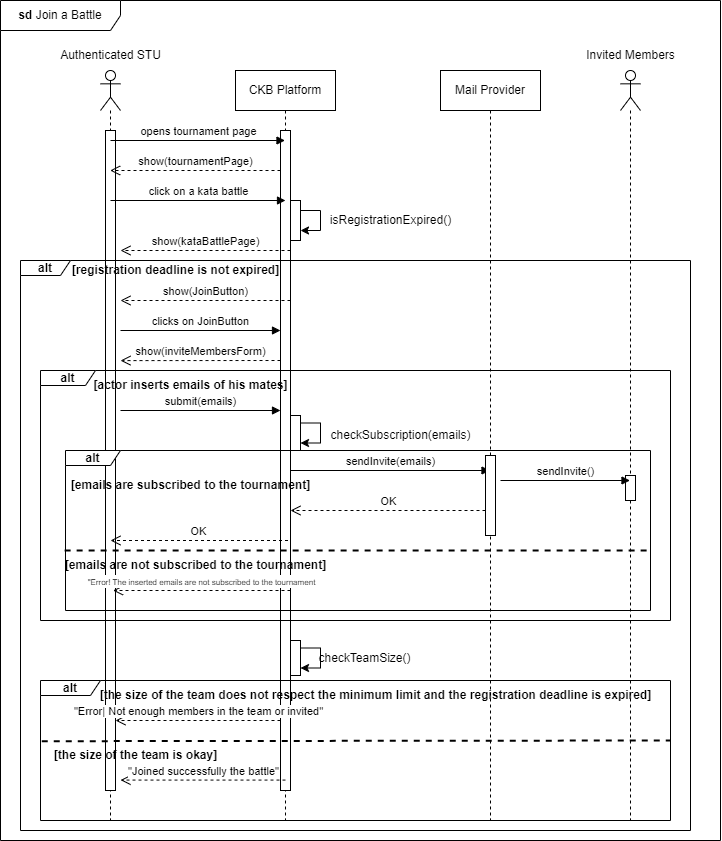
\includegraphics[width=1\textwidth]{images/sequence_diagrams/ClassDiagram-UC7-SequenceDiagram.png}
    \caption{Join a Battle Use Case}
    \label{fig:uc7}
\end{figure}
\begin{figure}[H]
    \centering
    %\includegraphics[width=1\textwidth]{images/sequence_diagrams/.png/...}
    \caption{\color{red} Join team Use Case}
    \label{fig:uc8}
\end{figure}
\begin{figure}[H]
    \centering
    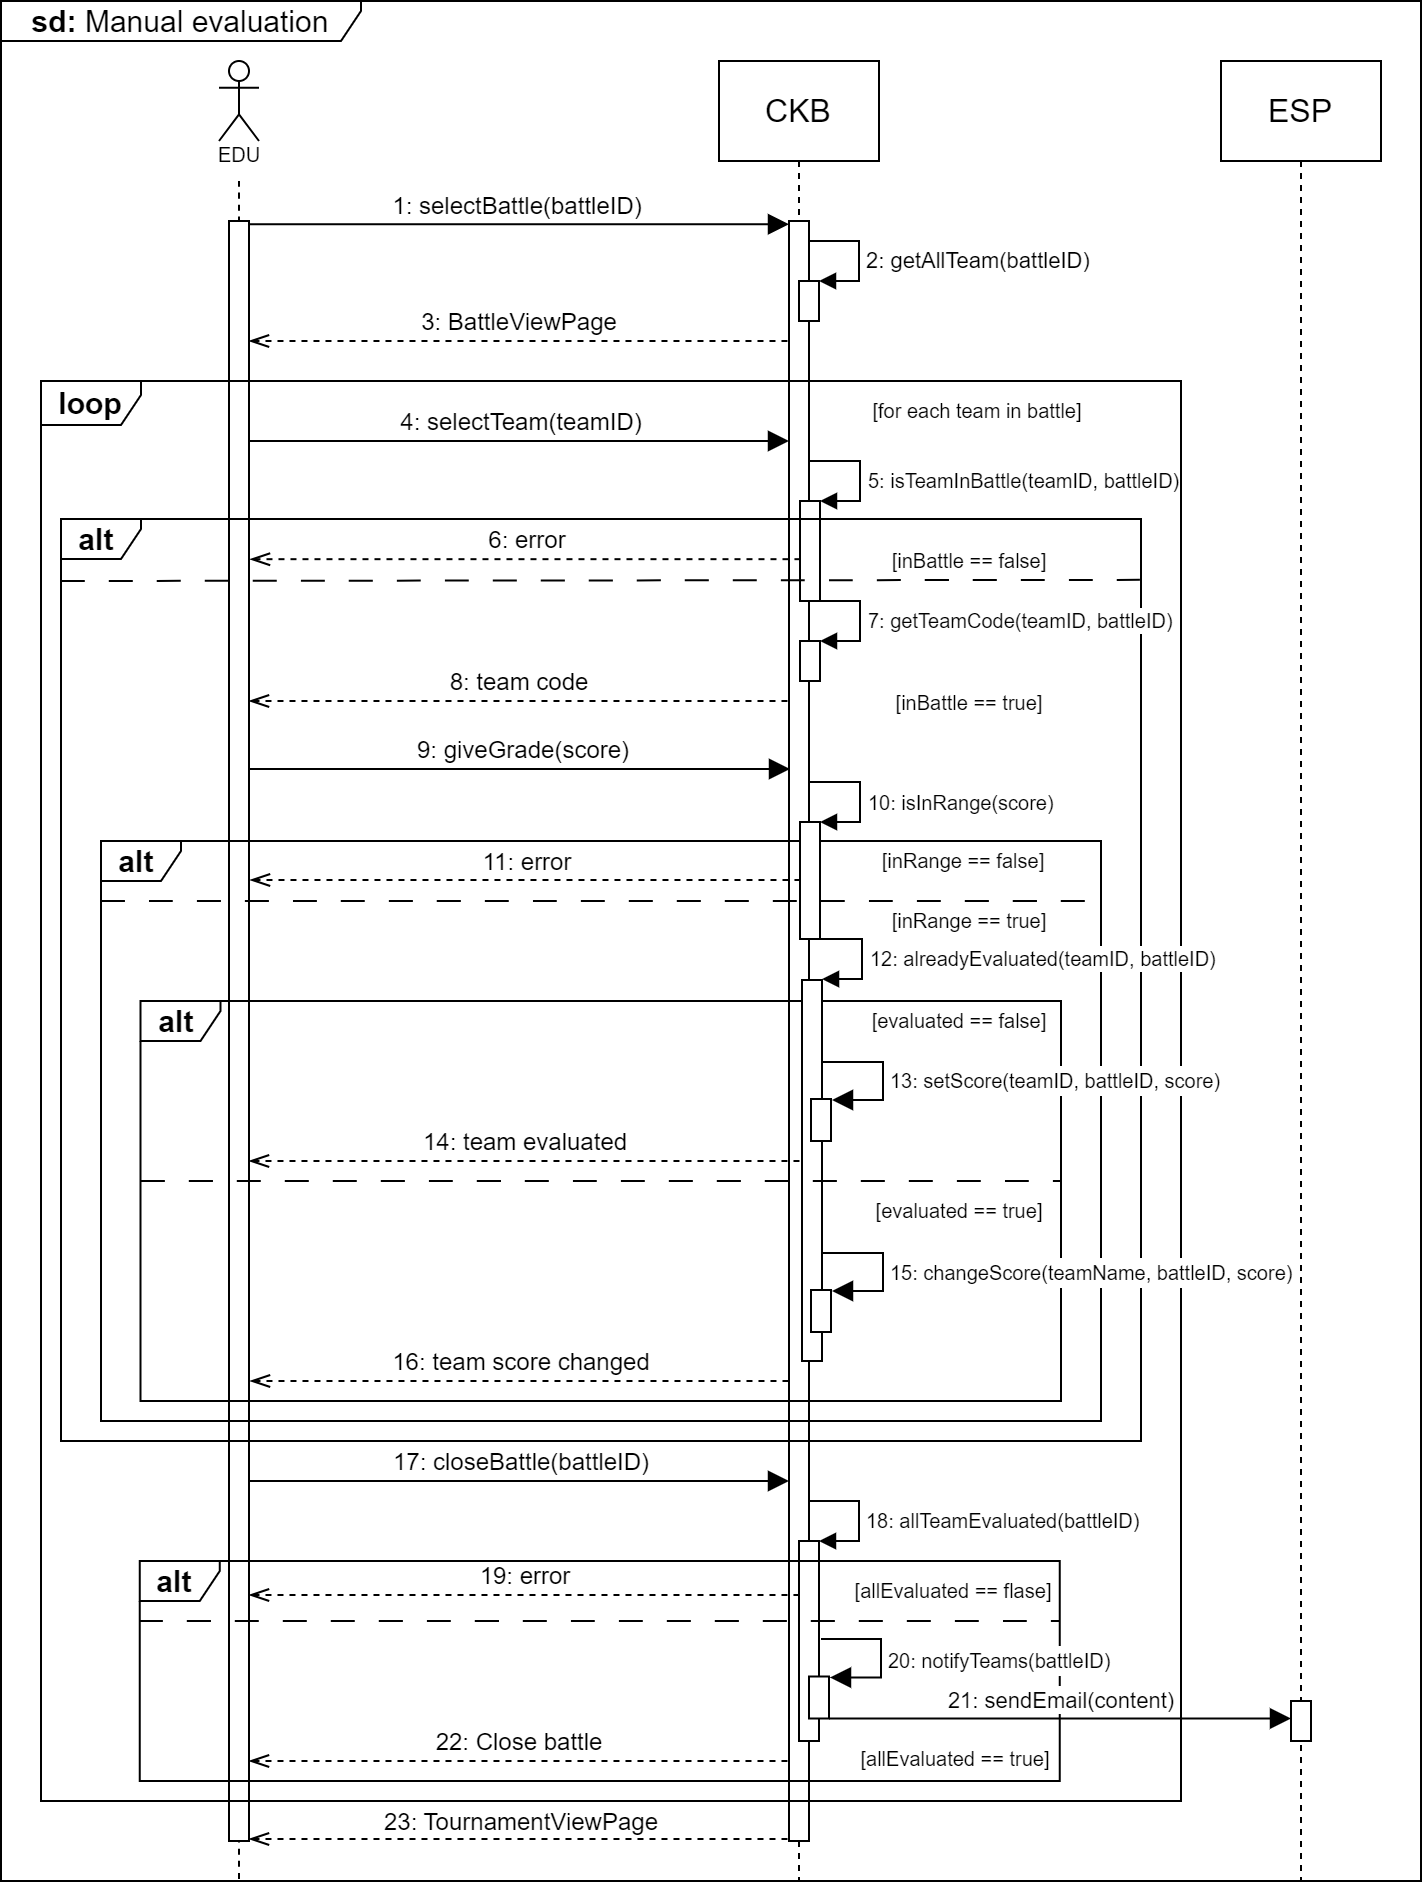
\includegraphics[width=1\textwidth]{images/sequence_diagrams/.png/Manual_Evaluation - UC9.png}
    \caption{Manual evaluation Use Case}
    \label{fig:uc9}
\end{figure}
\begin{figure}[H]
    \centering
    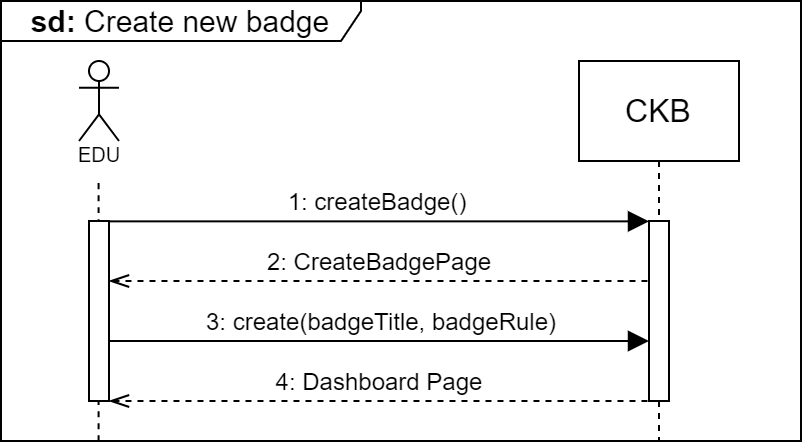
\includegraphics[width=1\textwidth]{images/sequence_diagrams/.png/Create_New_Badge - UC10.png}
    \caption{Create new badge Use Case}
    \label{fig:uc10}
\end{figure}
\begin{figure}[H]
    \centering
    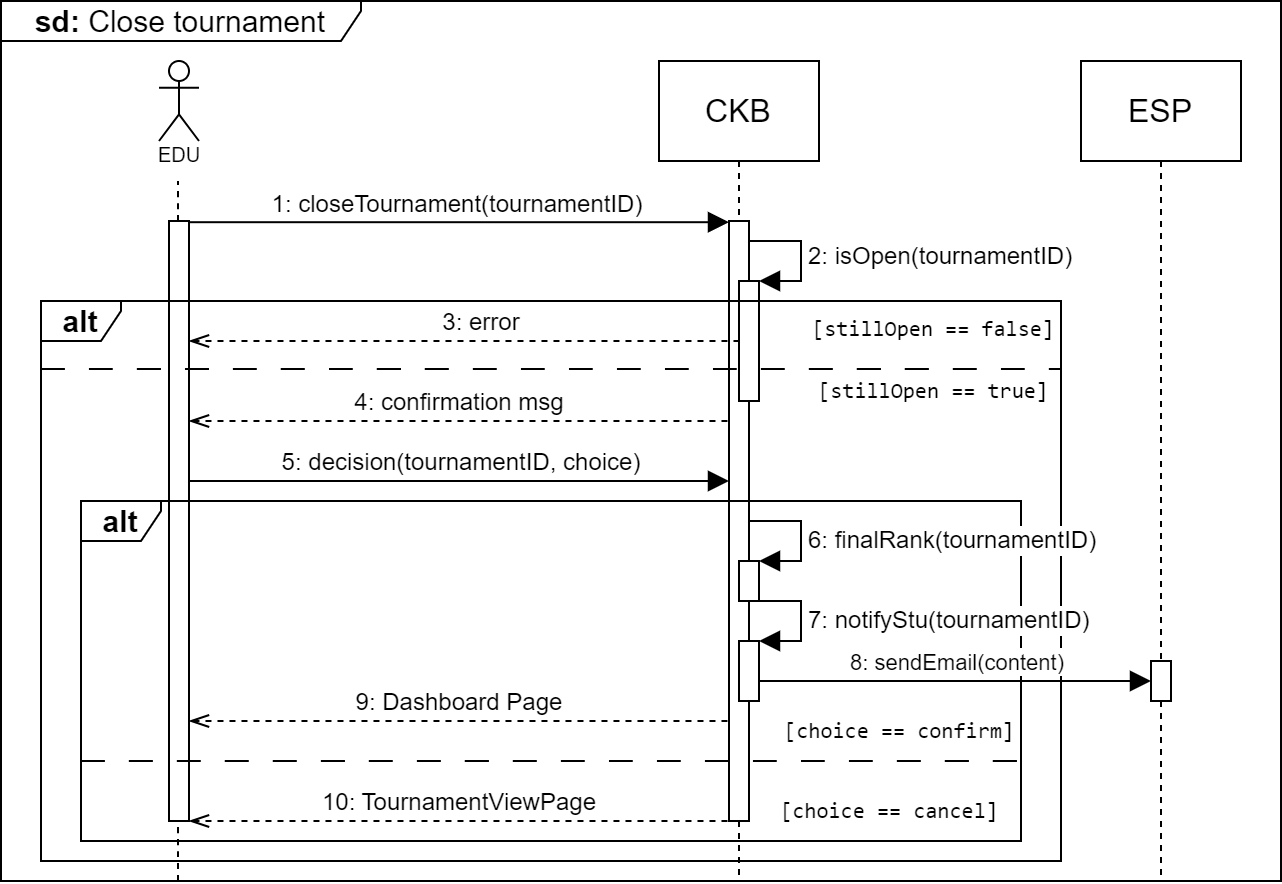
\includegraphics[width=1\textwidth]{images/sequence_diagrams/.png/Close_Tournament - UC11.png}
    \caption{Close tournament Use Case}
    \label{fig:uc11}
\end{figure}
\begin{figure}[H]
    \centering
    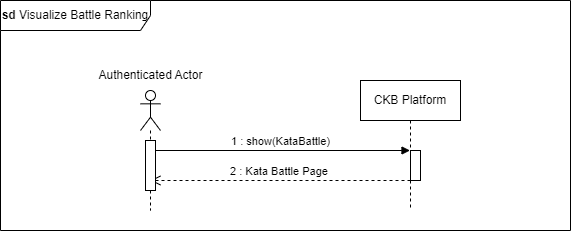
\includegraphics[width=1\textwidth]{images/sequence_diagrams/ClassDiagram-UC12-SequenceDiagram.png}
    \caption{View battle rank Use Case}
    \label{fig:uc12}
\end{figure}
\begin{figure}[H]
    \centering
    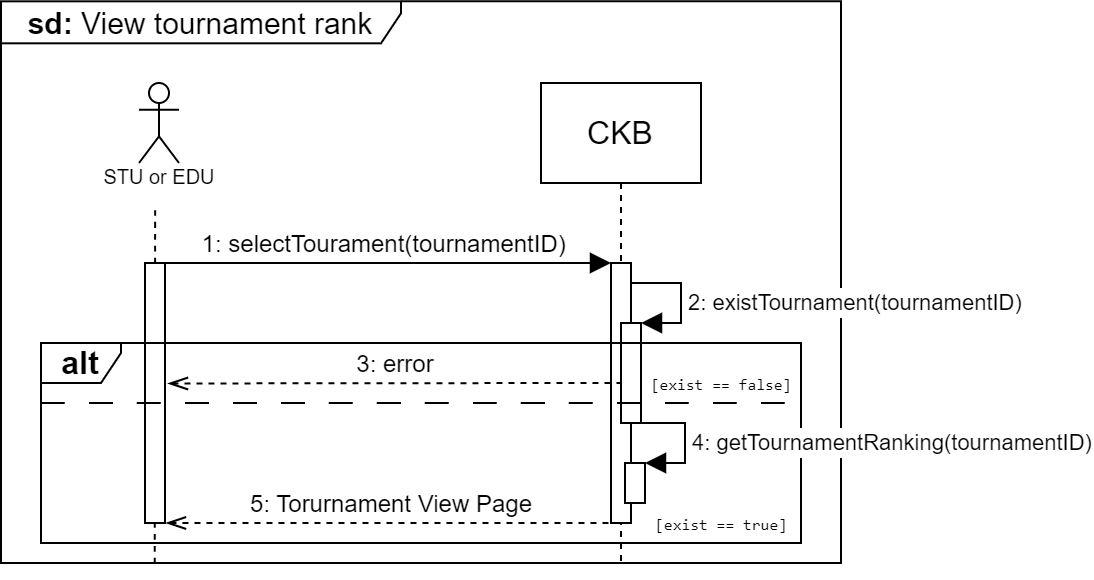
\includegraphics[width=1\textwidth]{images/sequence_diagrams/.png/View_Tournament_Rank - UC13.png}
    \caption{View tournament rank Use Case}
    \label{fig:uc13}
\end{figure}
\begin{figure}[H]
    \centering
    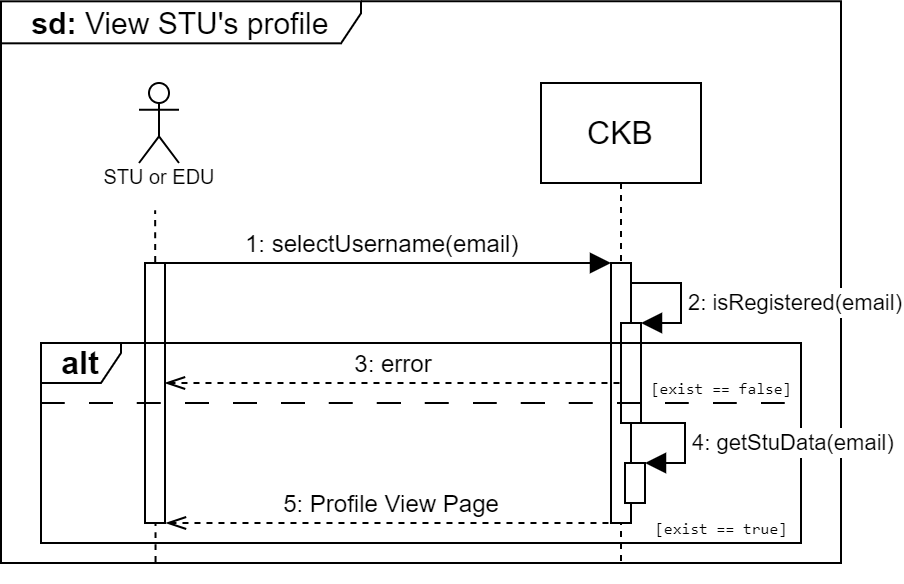
\includegraphics[width=1\textwidth]{images/sequence_diagrams/.png/View_STU's_Profile - UC14.png}
    \caption{View STU's profile Use Case}
    \label{fig:uc14}
\end{figure}
\begin{figure}[H]
    \centering
    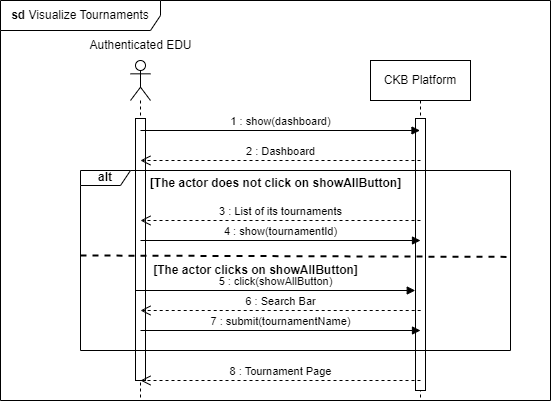
\includegraphics[width=1\textwidth]{images/sequence_diagrams/ClassDiagram-UC15.1-SequenceDiagram.png}
    \caption{View tournaments Use Case}
    \label{fig:uc15.1}
\end{figure}
\begin{figure}[H]
    \centering
    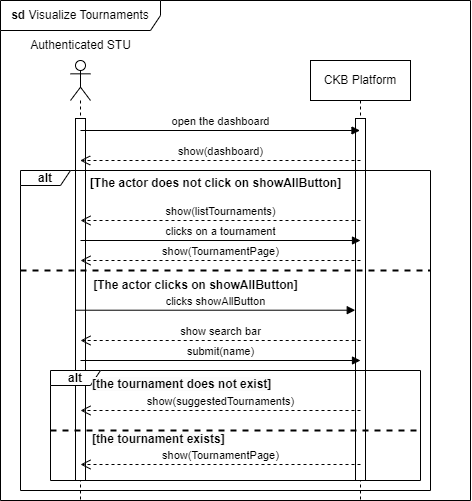
\includegraphics[width=1\textwidth]{images/sequence_diagrams/ClassDiagram-UC15.2-SequenceDiagram.png}
    \caption{View tournaments Use Case}
    \label{fig:uc15.2}
\end{figure}
\begin{figure}[H]
    \centering
    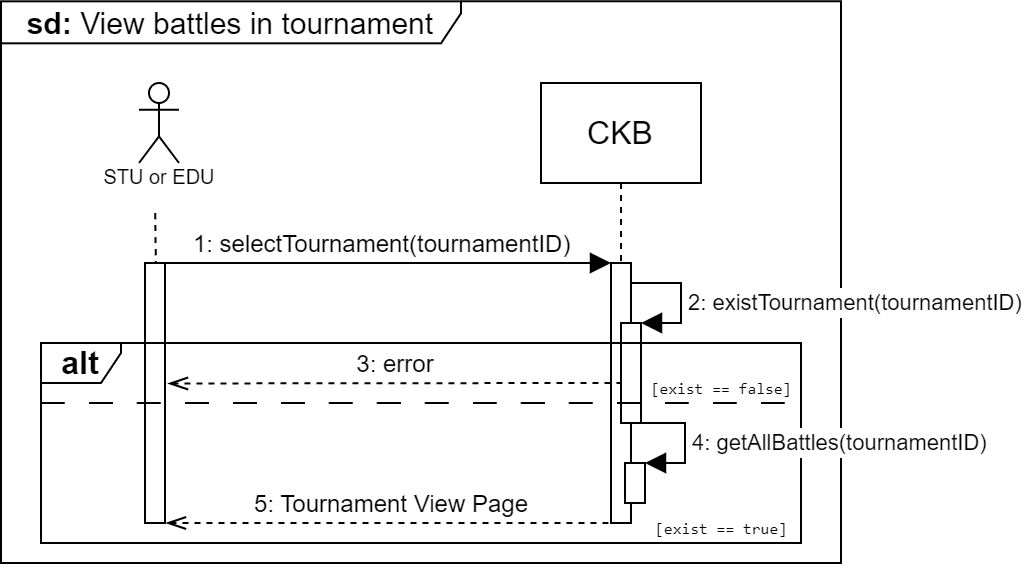
\includegraphics[width=1\textwidth]{images/sequence_diagrams/.png/View_Battles_in_Tournament - UC16.png}
    \caption{View battles in tournament Use Case}
    \label{fig:uc16}
\end{figure}
\begin{figure}[H]
    \centering
    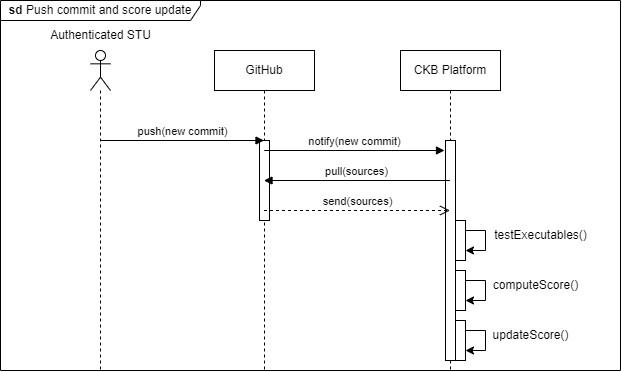
\includegraphics[width=1\textwidth]{images/sequence_diagrams/ClassDiagram-UC18-SequenceDiagram.png}
    \caption{Push commit and score updating Use Case}
    \label{fig:uc17}
\end{figure}
\begin{figure}[H]
    \centering
    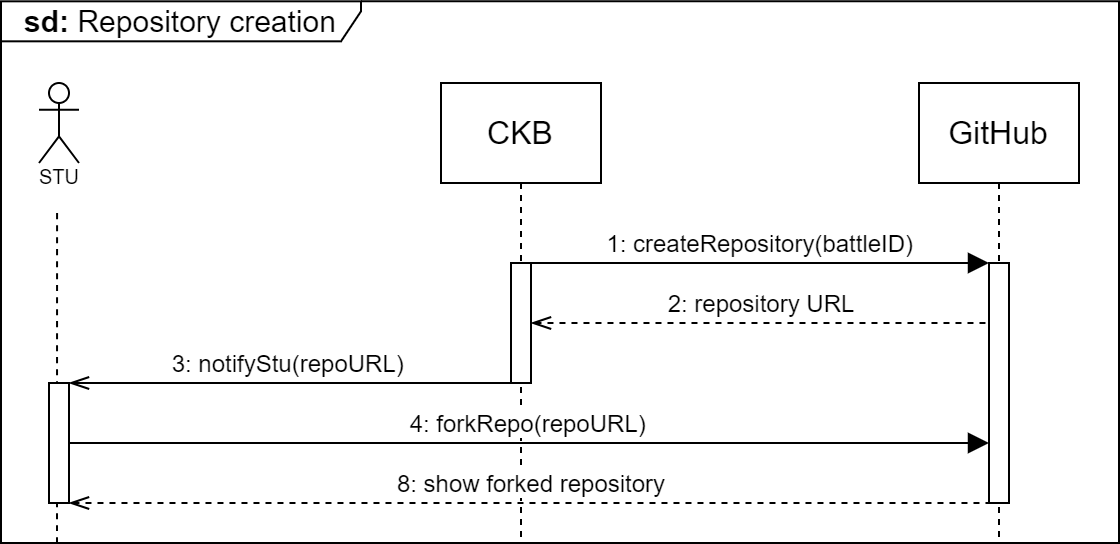
\includegraphics[width=1\textwidth]{images/sequence_diagrams/.png/Repository_Creation - UC18.png}
    \caption{Repository creation Use Case}
    \label{fig:uc18}
\end{figure}

\subsection{List of functional requirements}

\subsubsection*{EDU functional requirements}
\renewcommand{\arraystretch}{0.5}
\begin{longtable}[H]{l l p{12cm}}
    \hline
                 &        &                                                                                                                                                                                                                                                                          \\
    \textbf{ID}  & \vline & \textbf{Description}                                                                                                                                                                                                                                                     \\
                 &        &                                                                                                                                                                                                                                                                          \\\hline & & \\
    \textbf{R1}  & \vline & The software shall allow the unregistered EDUs to create an account.                                                                                                                                                                                                     \\
                 &        &                                                                                                                                                                                                                                                                          \\\hline & & \\
    \textbf{R2}  & \vline & The software shall allow the registered EDUs to log in.                                                                                                                                                                                                                  \\
                 &        &                                                                                                                                                                                                                                                                          \\\hline & & \\
    \textbf{R3}  & \vline & The software shall allow the authenticated EDUs to create new tournaments.                                                                                                                                                                                               \\
                 &        &                                                                                                                                                                                                                                                                          \\\hline & & \\
    \textbf{R4}  & \vline & The software shall allow an authenticated EDU to permit other authenticated colleagues to create battles in its tournament, those become owners of the tournament as much as who added them.                                                                             \\
                 &        &                                                                                                                                                                                                                                                                          \\\hline & & \\
    \textbf{R5}  & \vline & The software shall allow the authenticated EDUs to create coding battles in their tournaments by letting them upload the Code Kata, setting the minimum and maximum number of STUs per group, registration and final submission deadlines, and the score configurations. \\
                 &        &                                                                                                                                                                                                                                                                          \\\hline & & \\
    \textbf{R6}  & \vline & The software shall allow the authenticated EDUs to manually evaluate the work done by STUs subscribed to their own Code Kata battle.                                                                                                                                     \\
                 &        &                                                                                                                                                                                                                                                                          \\\hline & & \\
    \textbf{R7}  & \vline & The software shall allow the authenticated EDUs to see the sources produced by each team participating in their tournaments.                                                                                                                                             \\
                 &        &                                                                                                                                                                                                                                                                          \\\hline & & \\
    \textbf{R8}  & \vline & The software shall allow the authenticated EDUs to see the personal tournament score of each STU (which is the sum of all battle scores received in that tournament).                                                                                                    \\
                 &        &                                                                                                                                                                                                                                                                          \\\hline & & \\
    \textbf{R9}  & \vline & The software shall allow the authenticated EDUs to see a rank that measures how a STU's performance compares to other STUs in the context of that tournament.                                                                                                            \\
                 &        &                                                                                                                                                                                                                                                                          \\\hline & & \\
    \textbf{R10} & \vline & The software shall allow the authenticated EDUs to see the list of ongoing and finished tournaments as well as the corresponding tournament rank.                                                                                                                        \\
                 &        &                                                                                                                                                                                                                                                                          \\\hline & & \\
    \textbf{R11} & \vline & The software shall allow the authenticated EDUs to see the list of ongoing and finished battles as well as the corresponding battle rank within a tournament.                                                                                                            \\
                 &        &                                                                                                                                                                                                                                                                          \\\hline & & \\
    \textbf{R12} & \vline & The software shall allow an authenticated EDU to close a tournament iff it is one of the owners of that tournament.                                                                                                                                                      \\
                 &        &                                                                                                                                                                                                                                                                          \\\hline & & \\
    \textbf{R13} & \vline & When the authenticated EDU creates a tournament, the software shall allow it to define gamification badges concerning that specific tournament.                                                                                                                          \\
                 &        &                                                                                                                                                                                                                                                                          \\\hline & & \\
    \textbf{R14} & \vline & The software shall allow the authenticated EDU to create new badges and define new rules as well as new variables associated with them.                                                                                                                                  \\
                 &        &                                                                                                                                                                                                                                                                          \\\hline & & \\
    \textbf{R15} & \vline & The software shall allow all authenticated EDUs to visualize the badges created in CKB by other EDUs.                                                                                                                                                                    \\
                 &        &                                                                                                                                                                                                                                                                          \\\hline & & \\
    \textbf{R16} & \vline & The software shall allow all authenticated EDUs to visualize STUs' profile where they can see their collected badges, and some personal information.                                                                                                                     \\
                 &        &                                                                                                                                                                                                                                                                          \\
    \hline
    \caption{EDU's requirements}
\end{longtable}

\subsubsection*{STU functional requirements}

\renewcommand{\arraystretch}{0.5}
\begin{longtable}[H]{l l p{12cm}}
    \hline
                 &        &                                                                                                                                                                                                                       \\
    \textbf{ID}  & \vline & \textbf{Description}                                                                                                                                                                                                  \\
                 &        &                                                                                                                                                                                                                       \\\hline & & \\
    \textbf{R17} & \vline & The software shall allow the unregistered STUs to create an account.                                                                                                                                                  \\
                 &        &                                                                                                                                                                                                                       \\\hline & & \\
    \textbf{R18} & \vline & The software shall allow the registered STUs to log in.                                                                                                                                                               \\
                 &        &                                                                                                                                                                                                                       \\\hline & & \\
    \textbf{R19} & \vline & The software shall allow the authenticated STUs to form teams by inviting other STUs respecting the minimum and maximum number of STUs per group set for that battle.                                                 \\
                 &        &                                                                                                                                                                                                                       \\\hline & & \\
    \textbf{R20} & \vline & The software shall allow the authenticated STUs to join a team by an invite.                                                                                                                                          \\
                 &        &                                                                                                                                                                                                                       \\\hline & & \\
    \textbf{R21} & \vline & The software shall allow the authenticated STUs to subscribe to a tournament until a certain deadline.                                                                                                                \\
                 &        &                                                                                                                                                                                                                       \\\hline & & \\
    \textbf{R22} & \vline & The software shall allow the authenticated STUs subscribed to a coding battle to upload their work until the final submission deadline of that Code Kata battle.                                                      \\
                 &        &                                                                                                                                                                                                                       \\\hline & & \\
    \textbf{R23} & \vline & When the registration deadline of a battle expires, the software shall create a GitHub repository containing the Code Kata.                                                                                           \\
                 &        &                                                                                                                                                                                                                       \\\hline & & \\
    \textbf{R24} & \vline & The software shall send to all authenticated STUs who are members of subscribed teams to a battle the link to a GitHub repository containing the Code Kata.                                                           \\
                 &        &                                                                                                                                                                                                                       \\\hline & & \\
    \textbf{R25} & \vline & The software shall run the tests on executables pushed by a team, it shall also calculate and update the battle score of the corresponding team.                                                                      \\
                 &        &                                                                                                                                                                                                                       \\\hline & & \\
    \textbf{R26} & \vline & At the end of the consolidation stage of a specific battle \textit{'b'}, the software shall send a notification to all authenticated STUs participating to \textit{'b'} when the final battle rank becomes available. \\
                 &        &                                                                                                                                                                                                                       \\\hline & & \\
    \textbf{R27} & \vline & The software shall allow the authenticated STUs to see the list of ongoing and finished battles as well as the corresponding battle rank, iff they are part of the tournament.                                        \\
                 &        &                                                                                                                                                                                                                       \\\hline & & \\
    \textbf{R28} & \vline & The software shall allow all authenticated STUs to see the personal tournament score of each STU (which is the sum of all battle scores received in that tournament).                                                 \\
                 &        &                                                                                                                                                                                                                       \\\hline & & \\
    \textbf{R29} & \vline & The software shall allow all authenticated STUs to see a rank that measures how a STU's performance compares to other STUs in the context of that tournament.                                                         \\
                 &        &                                                                                                                                                                                                                       \\\hline & & \\
    \textbf{R30} & \vline & The software shall allow all authenticated STUs to see the list of ongoing and finished tournaments as well as the corresponding tournament rank.                                                                     \\
                 &        &                                                                                                                                                                                                                       \\\hline & & \\
    \textbf{R31} & \vline & The software shall notify all authenticated STUs involved in a closed tournament when the final tournament rank becomes available.                                                                                    \\
                 &        &                                                                                                                                                                                                                       \\\hline & & \\
    \textbf{R32} & \vline & The software shall allow all authenticated STUs to visualize other STUs' profile where they can see their collected badges, and some personal information.                                                            \\
                 &        &                                                                                                                                                                                                                       \\
    \hline
    \caption{STU's requirements}
\end{longtable}

\subsection{Traceability matrices}

\subsubsection*{Mapping of functional requirements on use cases}
\begin{center}
    \def\arraystretch{1.5}
    \begin{longtable}[H]{|c|l|}
        \hline
        \textbf{Use case} & \textbf{Functional requirements} \\ \hline
        UC1               & R1, R17                          \\ \hline
        UC2               & R2, R18                          \\ \hline
        UC3               & R3, R13                          \\ \hline
        UC4               & R5                               \\ \hline
        UC5               & R4                               \\ \hline
        UC6               & R21                              \\ \hline
        UC7               & R19, R20                         \\ \hline
        UC8               & R20                              \\ \hline
        UC9               & R6, R7, R26                      \\ \hline
        UC10              & R13, R14, R15                    \\ \hline
        UC11              & R12, R31                         \\ \hline
        UC12              & R11, R27                         \\ \hline
        UC13              & R8, R9, R10, R28, R29, R30       \\ \hline
        UC14              & R16, R32                         \\ \hline
        UC15              & R10, R30                         \\ \hline
        UC16              & R11, R27                         \\ \hline
        UC17              & R7, R22, R25                     \\ \hline
        UC18              & R22, R23, R24                    \\ \hline
    \end{longtable}
\end{center}

\subsubsection*{Mapping $D \wedge R \vDash G$}

\begin{center}
    \def\arraystretch{1.5}
    \begin{longtable}{p{0.5\textwidth}p{0.5\textwidth}}
        \specialrule{0.6mm}{1pt}{1pt}
        \multicolumn{2}{p{\textwidth}}{G1: Educators can create tournaments that involve coding battles to challenge students. }                                                                                           \\ % \specialrule{0.1mm}{1pt}{1pt}
        D2, D5, D6                    & R1, R2, R3, R4, R5, R6, R12, R13, R17, R18, R21, R22, R23, R24                                                                                                                     \\ \specialrule{0.6mm}{1pt}{1pt}

        \multicolumn{2}{p{\textwidth}}{G2: Provides educators with the ability to track student software development knowledge.}                                                                                           \\ % \specialrule{0.1mm}{1pt}{1pt}
        D2, D3, D4, D5, D6, D8        & R1, R2, R6, R7, R8, R9, R10, R11, R13, R14, R15, R17, R18, R21, R22, R24, R25                                                                                                      \\ \specialrule{0.6mm}{1pt}{1pt}

        \multicolumn{2}{p{\textwidth}}{G3: Students can improve software development skills by taking part in coding tournaments and battles where they must write programs.}                                              \\ % \specialrule{0.1mm}{1pt}{1pt}
        D1, D2, D3, D4,D5, D6, D7, D8 & R1, R2, R3, R4, R5, R6, R7, R13, R14, R16, R17, R18, R19, R20, R21, R22, R23, R24, R25, R26, R27, R28, R29, R30, R31, R32                                                          \\ \specialrule{0.6mm}{1pt}{1pt}

        \multicolumn{2}{p{\textwidth}}{G4: Coding battles enable students to enhance their soft skills, such as communication, collaboration, and time management, by creating a team and collaborating with the members.} \\ % \specialrule{0.1mm}{1pt}{1pt}
        D3, D5, D7, D8                & R5, R17, R18, R19, R20                                                                                                                                                             \\ \specialrule{0.6mm}{1pt}{1pt}
    \end{longtable}
\end{center}

\section{Performance Requirements}
To guarantee a good user experience, the system must:

\begin{itemize}
    \item Make sure the backend can grow as needed, respond quickly to changes, and balance the workload effectively.
    \item Be protected against DDoS attacks to keep the system safe and stable.
    \item Create a user-friendly, responsive front end.
          It should handle well even when the internet is not great, so users have a smooth experience.
    \item Send email notifications quickly, so users do not even notice the delay.
\end{itemize}

\section{Design Constraints}

\subsection*{Standards Compliance}
Since there are a lot of interactions between the various components of the system, it is important to follow some communication standards:
in particular, the system uses the REST architectural style to communicate between the frontend and the backend, and the data will be exchanged in JSON format.\\
Furthermore, the Source code of the application must be commented on and documented adequately.

\subsection*{Hardware Limitations}
The system is designed to be used on any device with a modern browser installed, so the only hardware limitation is the presence of a stable internet connection.

\section{Software System Attributes}
\subsection{Reliability}
Since some functionality of the system relies on external APIs, the system should not completely fail because of failure in one of those.\\
It is also important to avoid data loss through redundant storage methods.

\subsection{Availability}
In the event of an unplanned system downtime, all features should be restored as quickly as possible to minimize any inconvenience.
To prevent such occurrences, the CKB platform must have a reliable infrastructure, including redundant servers, to ensure continuous operation.
The aimed availability of the system is 3-nines availability (99.9\%), which means that the system can be down for less than 9 hours per year.\\
The system should also be able to handle a large number of concurrent users.

\subsection{Security}
Users of the system have distinct privileges according to their roles (student / educator), determined during the login process.\\
All data and information transferred and stored within the system are secured through robust encryption methods, such as HTTPS, ensuring data privacy and security.

\subsection{Maintainability}
The source code and associated documentation must include clear comments and should be consistently maintained.
During the design and development phases, emphasis should be placed on achieving modularity, minimizing coupling, and ensuring high cohesion between components.
This is especially crucial for both the front-end and back-end, allowing developers to make updates to the back-end seamlessly without causing any disruptions or noticeable changes for users.\\
To avoid inconvenience in solving any type of problem (e.g. server downtime), maintenance services are notified to all users with an advance notice of at least 36 hours.

\subsection{Portability}
Due to the fact that the CKB platform is a distributed system, and it does not rely on specific hardware or software, it can be used / accessed in multiple ways.